\documentclass{article}
\PassOptionsToPackage{numbers, compress}{natbib}
\usepackage[preprint]{neurips_2026}

% --- standard packages ---
\usepackage[utf8]{inputenc}
\usepackage[T1]{fontenc}
\usepackage[colorlinks=true,linkcolor=blue!70!black,citecolor=blue!70!black,urlcolor=blue!70!black]{hyperref}
\usepackage{url}
\usepackage{booktabs}
\usepackage{amsfonts}
\usepackage{nicefrac}
\usepackage{microtype}
\usepackage{xcolor}
\usepackage{graphicx}
\usepackage{subcaption}
\usepackage{amsmath}
\usepackage{amssymb}
\usepackage{amsthm}
\usepackage{algorithm}
\usepackage{algorithmic}
\usepackage{bm}
\usepackage{multirow}

% --- figure/table placement ---
\setcounter{topnumber}{1}
\setcounter{bottomnumber}{1}
\renewcommand{\topfraction}{0.5}

% --- theorem environments ---
\newtheorem{theorem}{Theorem}
\newtheorem{lemma}[theorem]{Lemma}
\newtheorem{proposition}[theorem]{Proposition}
\newtheorem{corollary}[theorem]{Corollary}
\theoremstyle{definition}
\newtheorem{definition}[theorem]{Definition}
\theoremstyle{remark}
\newtheorem{remark}[theorem]{Remark}

% --- custom commands ---
\newcommand{\vxi}{\bm{\xi}}
\newcommand{\vX}{\mathbf{X}}
\newcommand{\vm}{\mathbf{m}}
\newcommand{\vr}{\mathbf{r}}
\newcommand{\veps}{\bm{\epsilon}}
\newcommand{\R}{\mathbb{R}}
\DeclareMathOperator{\softmax}{softmax}
% Generated by code/experiments/generate_paper_tables.jl; do not edit.
\newcommand{\KunitzFobsFiveHundred}{0.581}
\newcommand{\KunitzFobsFiveHundredSD}{0.006}
\newcommand{\AttnMaxDevPts}{3.0}
\newcommand{\AttnMaxDevFamily}{$\omega$-Conotoxin}
\newcommand{\AttnMaxDevRho}{1}
\newcommand{\RelationIntercept}{0.77}
\newcommand{\RelationSlope}{-2.0}
\newcommand{\RelationRsq}{0.80}
\newcommand{\RelationLooSlopeMin}{-2.7}
\newcommand{\RelationLooSlopeMax}{-1.4}
\newcommand{\RelationLooRsqMin}{0.76}
\newcommand{\RelationLooRsqMax}{0.91}
\newcommand{\KunitzNaturalFraction}{0.323}
\newcommand{\KunitzSeparation}{0.20}
\newcommand{\SHThreeNaturalFraction}{0.600}
\newcommand{\SHThreeSeparation}{0.34}
\newcommand{\WWNaturalFraction}{0.164}
\newcommand{\WWSeparation}{0.11}
\newcommand{\HomeoboxNaturalFraction}{0.750}
\newcommand{\HomeoboxSeparation}{0.42}
\newcommand{\ForkheadNaturalFraction}{0.496}
\newcommand{\ForkheadSeparation}{0.17}
\newcommand{\ConotoxinNaturalFraction}{0.311}
\newcommand{\ConotoxinSeparation}{0.78}


\title{Conditioning Protein Generation via Hopfield Pattern Multiplicity}

\author{%
  Jeffrey D.~Varner \\
  R.F. Smith School of Chemical and Biomolecular Engineering\\
  Cornell University, Ithaca, NY 14850 \\
  \texttt{jdv27@cornell.edu} \\
}

\begin{document}

\maketitle

\begin{abstract}
% abstract.tex -- Abstract
Small protein-family alignments often contain a user-designated subset of interest but too
little labeled data for training a conditional generator; we address this regime by adding one
multiplicity ratio to the attention logits of a training-free stochastic-attention sampler,
continuously shifting generation from the full family toward the designated sequences. For
unit-norm memories, the resulting Boltzmann target is an exact Gaussian mixture with normalized
multiplicities as component weights, which separates exact latent conditioning from the
calibration gap introduced by dimensionality reduction, reconstruction, and sequence decoding.
Across five Pfam families and an $\omega$-conotoxin peptide family, the attention mass tracked
the analytic target while decoded single-position markers depended on subset separation; a
matched multiplicity-weighted profile-HMM benchmark transferred those marginal markers more
directly, whereas stochastic attention gave lower ESM2 pseudo-perplexity in the matched Kunitz
comparison. Curated seeding of 23 $\omega$-conotoxin accessions also produced diverse sequences
that retained the cysteine scaffold, Tyr13 marker, and several residue frequencies reported in
prior mutagenesis studies, generating experimentally testable candidates without establishing
binding.

\end{abstract}


\section{Introduction}
% introduction.tex
Generating novel protein sequences that fold correctly and perform a desired function is a
central goal of computational protein engineering. Several classes of methods now address this
problem. Deep generative models, including variational autoencoders~\cite{hawkinsHookerVAE2021},
autoregressive language models~\cite{madaniProGen2023}, and diffusion
models~\cite{alamdariProteinGeneration2023}, learn sequence distributions from large databases
and can produce diverse candidates, but require substantial training data and GPU resources.
Structure-conditioned inverse folding methods~\cite{dauparasProteinMPNN2022} design sequences for
a given backbone but require a target structure as input. Protein language
models~\cite{esmfold2022} trained on evolutionary databases can score or sample sequences, but
conditioning them on a specific functional property typically requires fine-tuning on labeled
data. Profile hidden Markov models (HMMs)~\cite{hmmer3} provide a standard training-free model
of family alignments. Sequence weights can shift their position-specific emission marginals
toward a designated subset, making a weighted profile HMM a direct comparator for the present
method. Profile HMMs do not model correlations between match-state emissions, whereas
stochastic attention samples a continuous representation of complete stored sequences. We
therefore compared the two methods under the same alignments, designation labels, and multiplicity ratios. For the
scarce-data regime considered here (families with tens to hundreds of members, typical of Pfam
seed alignments), models trained on the target family alone have limited training signal.
Pretrained models are not restricted in this way, since they draw on sequence data beyond the
target family.

Stochastic attention (SA) was developed for the scarce-data regime where traditional methods struggle due to limited training data~\cite{varnerSAProtein2026}. Stochastic attention treats the energy function of a modern Hopfield network, constructed directly from a small family alignment, as a Boltzmann density and samples from it using Langevin dynamics. The method requires no training, runs on a laptop, and produces sequences that preserve family-level amino acid composition, per-position conservation, and predicted three-dimensional fold. A key
limitation, however, is that SA treats all sequences in the alignment equally. Every family
member contributes the same weight to the energy landscape, so the sampler explores the full
family distribution without preference for any functional subset. In practice, experimentalists
often want something more specific: not just a plausible Kunitz domain, but a Kunitz domain
that \emph{inhibits trypsin}; not just a plausible SH3 domain, but one that binds a
particular proline-rich motif. The members of a family alignment share a fold but differ in
function, and the residues that carry the difference occupy only a few positions. A sampler
that reproduces the family distribution faithfully therefore reproduces its variation at those
positions, producing the functionally relevant residue only as often as it appears in the
alignment. This raises the question of how to condition the generative process on a functional
subset without retraining.

In this study, we answered that question with multiplicity weighting. Stochastic attention
encodes each aligned sequence as a column in a memory matrix. At each step the sampler
computes attention weights over these stored sequences and moves toward their weighted average.
A bias added to the attention scores makes it spend more time near selected sequences. We
assigned a multiplicity weight $r_k > 0$ to each stored sequence and added $\log r_k$ to its
attention score before the softmax normalization. All designated sequences share one weight and all
background sequences share another, so a single number, the multiplicity ratio $\rho$ between
the two weights, controls the strength of the bias: $\rho = 1$ recovers standard SA (no
preference), while increasing $\rho$ shifts generation toward the designated subset. 
The method is agnostic to what the designated subset represents (binding, thermostability, organism of origin); it simply biases the sampler toward the sequences the user points to. 
The same multiplicity-weighted mechanism has also been applied to synthetic patient generation
from small longitudinal clinical cohorts~\cite{varnerSAPatient2026}, so the conditioning is not
specific to sequence data. We compared multiplicity weighting against the obvious alternative,
hard curation, which builds the memory matrix from the designated sequences alone and leaves
the rest of the family out. Those discarded sequences are what show which
positions the fold holds fixed and which are free to vary, so dropping them leaves the sampler
with far fewer examples to work from. We tested both on five
Pfam protein families (Kunitz, SH3, WW, Homeobox, and Forkhead domains) spanning a range of
family sizes ($K = 55$--$420$) and designated-subset geometries. Hard curation retained the
selected marker completely from as few as three designated inputs. Those inputs were chosen
because they carry the marker, so recovering it demonstrated control over the sampler and not
that the generated sequences had the function the marker stands for. The multiplicity weights,
by contrast, enter the sampler as a simple logit bias, preserving the analytic score function and
$\mathcal{O}(dK)$ per-step cost of the original method. The conditioning has two stages, and only the
first was exact. Inside the sampler, the mean attention mass on the designated patterns matched
the fraction that $\rho$ sets to within \AttnMaxDevPts{} percentage points at worst
(\AttnMaxDevFamily{}, $\rho=\AttnMaxDevRho$) across the canonical replicated sweeps. Turning
those continuous states back into discrete sequences cost part of that conditioning: after
finite-temperature sampling, reconstruction from unit-normalized principal component analysis
(PCA) coordinates, and argmax decoding, the fraction of generated sequences carrying the marker
could fall below the attention mass the sampler had placed on the designated set. We termed that
shortfall the calibration gap and examined it against a simple geometric quantity, the
separation index $S$, which measures how well PCA separates designated from background
sequences. Multiplicity weighting therefore offers a practical route to
conditioning generative models in the scarce-data regime, and the calibration gap is the
quantity anyone applying such conditioning should measure before trusting it.


\section{Results}
% results.tex

We evaluated SA on six protein families with different sizes, functions, and PCA-space
geometries (Table~\ref{tab:cross-family}). Five were Pfam seed families: Kunitz
(PF00014, $K=99$), SH3 (PF00018, $K=55$), WW (PF00397, $K=420$), Homeobox
(PF00046, $K=136$), and Forkhead (PF00250, $K=246$). We used these families to test
hard curation and multiplicity-weighted conditioning. Data-selected single-position markers
defined their designated subsets. Prior literature motivated the residue classes where
available, but the markers are not direct activity labels. We also studied the
$\omega$-conotoxin O-superfamily ($K=74$, curated from SwissProt) as a peptide example
associated with the Cav2.2 calcium channel.

For each family, we split the sequences into designated and background subsets. We then built
the conditioned memory matrices and generated sequences at the entropy-crossover inverse
temperature $\beta^{*}$. The separation index $S$ measures PCA separation between the two
subsets. It ranged from \WWSeparation{} for WW to \HomeoboxSeparation{} for Homeobox. This
range allowed us to compare conditioning across different PCA geometries.

\paragraph{Hard curation and marker retention.}
We restricted the memory matrix to a K/R-at-P1-positive subset of Kunitz domains
(PF00014; $K=99$ sequences, $L=53$ aligned positions) and tested whether the selected
sequence marker transfers to generated sequences (Fig.~\ref{fig:scaling}). Kunitz domains are
serine protease inhibitors. The P1 residue at the primary contact site influences target
specificity.
Lys or Arg at P1 is associated with trypsin specificity~\cite{laskowskiProteinInhibitors1980},
but is not by itself an activity measurement for every sequence. We designated the 32 sequences
with K/R at P1 as the marker-positive subset ($K_{\mathrm{des}} = 32$) and the remaining 67 as
marker-negative background ($K_{\mathrm{bg}} = 67$). We built a separate memory matrix for
each group and selected $\beta^{*}$ from the entropy-crossover onset. Each condition produced
930 sequences from 30 chains run for 5{,}000 steps and thinned after burn-in.
All designated-subset-conditioned sequences had K/R at P1. No background-conditioned
sequence did. Full-family generation produced 38\% K/R, compared with 32\% in the input
family. Complete K/R retention is expected because the designated input was selected on this
marker. It is not independent evidence of trypsin inhibition.
Sequence-level inspection showed that the top K/R-positive-subset-conditioned sequences
preserved all 11 highly conserved positions, all six cysteines, and K/R at P1. They contained
19--26 substitutions, mainly at variable sites. Per-position Shannon entropy correlated with
the stored MSA for both full-family generation ($r = 0.988$) and K/R-positive-subset
conditioning ($r = 0.932$). The largest change occurred at P1, where conditioning restricted
the residues to K/R (Fig.~\ref{fig:sequence-analysis}).

We next varied the designated input size. We sampled
$K_{\mathrm{des}} \in \{3, 5, 8, 10, 15, 20, 25, 32\}$ Kunitz K/R-positive sequences and
used three replicates per size. P1 marker retention was 100\% at every size, including
$K_{\mathrm{des}}=3$. Pairwise sequence diversity increased from 0.35 at
$K_{\mathrm{des}}=3$ to 0.50 at $K_{\mathrm{des}}=32$. Over the same range, KL divergence
decreased from 0.070 to 0.009 (Fig.~\ref{fig:scaling}). Smaller input sets define a narrower
PCA subspace and therefore produced less diverse libraries. These results show marker
retention from small designated inputs, with diversity increasing as more inputs were added.

\paragraph{Multiplicity-weighted conditioning and the calibration gap.}
We tested multiplicity-weighted generation on the Kunitz family ($K = 99$,
$K_{\mathrm{des}} = 32$ K/R-positive sequences, $K_{\mathrm{bg}} = 67$ background),
sweeping $\rho$ from 1 (standard SA, no bias) to 500 in the canonical replicated
analysis (Fig.~\ref{fig:phase-transition}, Table~\ref{tab:per-family-rho}). For each $\rho$, we
computed the multiplicity vector $\vr$. We then found $\beta^{*}(\vr)$ from the
entropy-crossover onset of the weighted attention distribution. We ran five independent
replicates of 20 chains, with 620
retained samples per replicate. At each $\rho$, we recorded the mean attention weight on
designated patterns, $\bar{a}_{\mathrm{des}}$. We also recorded the decoded K/R fraction at
P1, $f_{\mathrm{obs}}$. Across all six canonical replicated sweeps, the largest absolute
attention deviation was \AttnMaxDevPts{} percentage points
(\AttnMaxDevFamily{}, $\rho=\AttnMaxDevRho$), showing close but not exact finite-sample
agreement with the target mixture fraction. However, the decoded marker fraction told a
different story. For Kunitz, P1~K/R reached
\KunitzFobsFiveHundred{} $\pm$ \KunitzFobsFiveHundredSD{} at $\rho=500$, far short of the
$f_{\mathrm{eff}} = 0.996$
that the attention weights achieved. This discrepancy between latent designated mass and the
decoded marker marginal is the calibration gap. As
Eq.~\ref{eq:decoder-pushforward} shows, it reflects both false negatives and
false positives under the complete latent-to-sequence map. Sequence diversity decreased
from 0.56 to 0.51 over this range. KL divergence increased from 0.007 to 0.017. The entropy crossover
$\beta^{*}$ shifted from 4.4 at $\rho=1$ ($K_{\mathrm{eff}} = 99$) to 9.3 at
$\rho=1{,}000$ ($K_{\mathrm{eff}} = 32.1$). The entropy curves shifted to the right as
$\rho$ increased (Fig.~\ref{fig:phase-transition}).

To examine this gap, we measured three layers of the signal chain
(Eq.~\ref{eq:gap-decomp}) over 17 values of $\rho$ from 1 to 1{,}000, with five replicates
per value. The measurements were designated attention mass
$\bar{a}_{\mathrm{des}}$, continuous reconstructed K/R probability
$f_{\mathrm{soft}}$, and decoded K/R fraction $f_{\mathrm{obs}}$. The attention gap remained
small. The PCA term was the largest component. The value of $f_{\mathrm{soft}}$ stayed near
0.27 and varied by less than 0.04 over the full range of $\rho$. The argmax term was negative
($\approx-0.25$), so discrete decoding recovered some signal lost during PCA reconstruction.
Even with 99.8\% of the attention on designated patterns, the continuous reconstruction did
not resolve K from G at P1. This variation was not well represented by the leading
$d=80$ principal components. The Kunitz split had separation index
$S=\KunitzSeparation$, which indicates partial PCA overlap.

\paragraph{Exact-equilibrium benchmark.}
The closed-form Gaussian-mixture target permits independent equilibrium sampling without
a Markov chain. We compared 1{,}640 exact draws with 1{,}640 retained ULA states at
$\rho\in\{1,10,500\}$, using the same $\beta^{*}$ and decoder in each comparison. At
$\rho=500$, the exact designated-component probability was
$f_{\mathrm{eff}}=0.996$, while the decoded P1~K/R fraction was 0.604 under exact
sampling and 0.597 under ULA. The amino acid composition divergence
$D_{\mathrm{KL}}(\text{exact} \parallel \text{ULA})$ between the two decoded libraries
was $1.19\times10^{-4}$. Across all three conditions, exact
and ULA MAP-designated basin occupancies differed by at most 0.026, and the decoded
P1~K/R fractions differed by at most 0.016. The full comparison is provided in the
Supporting Information. These results show that the calibration gap persists at
exact equilibrium, indicating that finite-step ULA discretization and mixing error were not
the main source of the gap.

\paragraph{Cross-family marker analysis and the separation index.}
We repeated the multiplicity analysis on four additional Pfam families. The SH3 split
(PF00018; $K=55$) used a data-selected Trp marker. The WW split
(PF00397; $K=420$) used a data-selected middle-third residue. The Homeobox split
(PF00046; $K=136$) used a data-selected Gln marker. The Forkhead split
(PF00250; $K=246$) used a data-selected His/Asn marker. Together with Kunitz, these
families had distinct PCA-space geometries
(Table~\ref{tab:cross-family}, Table~\ref{tab:per-family-rho}). Their calibration gaps varied
inversely with separation overall, but not monotonically
(Fig.~\ref{fig:separation-vs-gap}). An exploratory unweighted fit across the five Pfam
families yielded
$\Delta \approx \RelationIntercept{} \RelationSlope\,S$ with $R^{2}=\RelationRsq$.
Leave-one-family-out sensitivity was substantial: slopes ranged from
\RelationLooSlopeMin{} to \RelationLooSlopeMax{} and $R^{2}$ from
\RelationLooRsqMin{} to \RelationLooRsqMax{}. The $\omega$-conotoxin point was displayed as
an external comparison and was not included in the Pfam fit. These data show a preliminary
association, not a prospective threshold or decision rule. The attention weights tracked
$f_{\mathrm{eff}}$ closely in all six families. Thus, the multiplicity-weighted energy reached
its target latent mass despite the downstream calibration gap. Hard curation achieved
100\% marker retention in every family, independent of the separation index. This result is
expected because its PCA basis contains only the designated subset.

We also tested whether increasing $\beta$ beyond $\beta^{*}$ transferred more marker signal
through the PCA representation. We swept $\beta/\beta^{*}$ from 0.5 to 3.0 at
$\rho = 10$, 50, and 200 on the Kunitz domain. Higher $\beta$ increased the P1~K/R
fraction and reduced diversity. At $\rho = 200$ and $\beta = 3\beta^{*}$, P1~K/R
reached 0.71, compared with 0.61 at $\beta^{*}$. Diversity decreased from 0.53 to 0.46.
Thus, $\rho$ and $\beta/\beta^{*}$ provide separate controls for marker retention and diversity.

\paragraph{The hard mask as the $\rho \to \infty$ endpoint.}
Hard attention masking sets the background attention mass to zero. It is the
$\rho \to \infty$ endpoint of the multiplicity axis on the full-family basis. It also gives
$\Delta_{\mathrm{attn}} = 0$ in Eq.~\ref{eq:gap-decomp}
(Table~\ref{tab:mask-recovery}).

We held the mask fixed and swept $\beta$ to measure the decode-limited recovery ceiling.
The P1~K/R fraction increased from 0.46 at $\beta = 2$ to 1.00 at $\beta = 512$
without a plateau (Fig.~\ref{fig:mask-betasweep}). Thus, the residual decode gap
$\Delta_{\mathrm{PCA}} + \Delta_{\mathrm{argmax}}$ decreased as retrieval sharpened.
At matched $\beta$, hard masking recovered more marker signal than finite-$\rho$ weighting.
The difference was 0.085 (SE 0.028) at $f_{\mathrm{eff}} = 0.5$ and 0.053
(SE 0.029) at $f_{\mathrm{eff}} = 0.7$. It decreased to 0.003 (SE 0.030) at
$f_{\mathrm{eff}} = 0.99$, where the mask and strongest finite-$\rho$ condition coincided.

Hard masking removes the background components and raises the intended designated mass from
$f_{\mathrm{eff}}$ to one. Matched-$\beta$ comparisons therefore have different intended
masses. Their difference should decrease as $f_{\mathrm{eff}}$ approaches one. Attention
realized the intended mass in each condition to within a fraction of a percent
($\Delta_{\mathrm{attn}} \approx 0$). A 0.5 difference in intended mass produced a
0.085 difference (SE 0.028) in observed marker fraction. The latent-to-sequence map
attenuated the response through noise, PCA reconstruction, and argmax decoding.
Both retrieval sharpness $\beta$ and conditioning strength $\rho$ affected recovery.
At high $\beta$, novelty decreased from 0.42 at the mask's $\beta^{*}$ to 0.16 at
$\beta = 512$ (Table~\ref{tab:mask-recovery}). Hard curation reached complete marker
retention at low $\beta$ with novelty of 0.32. Its subset-only basis retains designated
variation that the leading full-family components blur.

\paragraph{Application to a Cav2.2-associated $\omega$-conotoxin subset.}
We used the $\omega$-conotoxin O-superfamily to test curated conditioning beyond classical
protein domains (Table~\ref{tab:conotoxin-pharmacophore}, Fig.~\ref{fig:conotoxin-loop}).
These peptides come from cone snails and are rich in disulfide bonds. They block
voltage-gated calcium channels, including Cav2.2 in sensory neurons
~\cite{omegaConotoxinSAR2006}. Cav2.2 contributes to pain
signaling between peripheral nociceptors and the spinal cord. The family includes
$\omega$-conotoxin MVIIA (ziconotide), an approved non-opioid analgesic for intractable
pain~\cite{ziconotideReview2004}. Prior modeling of ATP-gated calcium dynamics in dorsal root
ganglion neurons also identified Cav2.2 as part of the pain signaling network
~\cite{songModelingAnalysis2009}.

Tyr13 is a reported Cav2.2 marker in MVIIA numbering. Its hydroxyl group contacts the channel
pore, and substitution of this residue abolishes binding. Basic residues distributed across
the peptide also contribute to electrostatic complementarity with the channel entrance.
We compiled 74 SwissProt $\omega$-conotoxin sequences and aligned them with
MAFFT~\cite{mafft2013}. Gap filtering retained 26 positions. The study's curated
Cav2.2-associated input list designated 23 accessions. The remaining 51 sequences
form a background set for conditioning and are not asserted to be nonbinders. An accession-level
audit records which designations have activity metadata in the repository and which are supported
only by the input list.

We ran two SA experiments with 50 chains, 5\,000 steps, and $\alpha = 0.01$. Each
condition generated 1\,550 sequences. One used the full family
($K = 74$, $\beta^{*} = 3.23$), and the other used only the designated accessions
($K = 23$, $\beta^{*} = 2.72$). Tyr occurred at the marker position in 33.8\% of the
full-family input and 46.9\% of full-family generation. It occurred in 82.6\% of the
designated input and 98.3\% of designated-subset generation
(Table~\ref{tab:conotoxin-pharmacophore}).

Accession designation and Tyr13 are distinct labels. They agree for 64 of 74 stored
sequences (86.5\%). The designated set contains 19 marker-positive sequences, and the
background contains six. We therefore report designation conditioning and Tyr13 recovery
separately. Designated-subset generation contained 20.1\% Lys or Arg, compared with
19.7\% in its input. Full-family generation contained 12.0\%, consistent with the lower
K/R content of the full-family input.

Per-position frequency heatmaps were similar for the designated input and its generated
sequences (Fig.~\ref{fig:conotoxin-loop}). Tyr13, the conserved Cys framework, and
variable-loop diversity were retained. The residual heatmaps showed small changes across
positions. Sequence-level analysis gave the same pattern
(Fig.~\ref{fig:conotoxin-sequence-analysis}). The five highest-pLDDT sequences retained
all six highly conserved positions, all six cysteines, and Tyr at the marker. They contained
5--11 substitutions at variable sites. The entropy correlation was $r = 0.745$ for
designated-subset generation and $r = 0.997$ for full-family generation. The lower
designated-subset value reflects reduced variation at co-varying loop positions.

We also compared 12 positions with published structure--activity relationship observations
(Table~\ref{tab:sar-agreement}). Designated-subset generation retained Tyr13 at 98.3\%.
It retained all six disulfide-forming cysteines at frequencies of at least 97.4\%. These
cysteines are invariant in the designated input. Designated-subset generation raised the
frequency of basic residues at loop~2 positions reported as important for channel
interaction (Arg10: 82.3\% K/R against 69.6\% in the designated input) and at
position~21 (66.2\% K/R against 47.8\%). It exceeded full-family generation at every
reported position outside the disulfide framework, where both conditions sat at or
near 1.00. The generated library therefore enriched several residues reported by
prior mutagenesis. These frequencies do not test mutation effects in the generated backgrounds
~\cite{kimTyr13Essential1995,satoBasicResidues1993,lewisConotoxinSAR2012}.
The top three designated-subset sequences had predicted disulfide-constrained loop
architectures consistent with an inhibitor cystine-knot-like fold
(Fig.~\ref{fig:fold-superposition}). Curated conditioning transferred sequence statistics
from the 23 designated accessions to the generated library. Sequence generation did not
require retraining or the Cav2.2 target structure.

\paragraph{AlphaFold2 multimer complex prediction.}
We compared complex-level predictions for SA-generated and natural $\omega$-conotoxins using
ColabFold AlphaFold2-multimer with the Cav2.2 pore-domain target
(Table~\ref{tab:docking-validation}). SA designated-subset ($n=10$; pTM
$0.221\pm0.007$, iPTM $0.105\pm0.008$, and interface pLDDT $37.2\pm5.4$).
The SA full-family values were $0.219\pm0.008$, $0.104\pm0.007$, and
$38.2\pm4.0$ ($n=10$). Natural controls had values of $0.228\pm0.004$,
$0.108\pm0.007$, and $40.7\pm3.5$ ($n=5$). All groups received low-confidence
complex predictions. Exact permutation tests detected no group
difference on the four reported metrics (all $p>0.05$), but these tests do not establish
equivalence or preserved binding geometry. Experimental complex structures and binding assays
are required to evaluate Cav2.2 interaction.

\paragraph{Model-based structure and sequence evaluation.}
We predicted folds for 50 sequences from each source (stored, full-family SA,
K/R-positive SA, K/R-negative SA, and HMM baseline) using ESMFold and computed TM-scores
against the experimental Kunitz domain structure (1BPI, chain~A) to compare
model-predicted structure summaries (Table~\ref{tab:structure-validation}).
SA-generated and stored sequences had similar model scores. Mean pLDDT was
$90.4 \pm 1.2$ for SA full-family, $90.7 \pm 1.1$ for SA K/R-positive, and
$89.3 \pm 3.2$ for stored sequences. All SA sequences exceeded the pLDDT $>70$
threshold. Their mean TM-scores were $0.84 \pm 0.01$, $0.83 \pm 0.01$, and
$0.83 \pm 0.03$, respectively (Fig.~\ref{fig:fold-superposition}). HMM-emitted
sequences had lower and more variable model scores. Their mean pLDDT was
$60.4 \pm 13.1$, with 20\% above the threshold, and their mean TM-score was
$0.60 \pm 0.19$ (Table~\ref{tab:structure-validation}).

AlphaFold2-ptm predictions via ColabFold gave similar summaries
~\cite{jumperHighlyAccurate2021,mirdita2022colabfold}. Kunitz TM-scores were
$0.83$--$0.85$ with pLDDT of $93$--$95$. The shorter $\omega$-conotoxins had
TM-scores of $0.35$--$0.47$ with pLDDT of $68$--$79$
(Table~\ref{tab:af2-validation}).

We used ESM2-650M masked marginal scoring to assess sequence plausibility. The resulting
pseudo-perplexity values were $4.78 \pm 0.64$ for SA full-family, $4.72 \pm 0.60$ for
SA K/R-positive, and $4.97 \pm 0.98$ for stored sequences. HMM-emitted sequences
had a value of $16.1 \pm 4.2$ (Table~\ref{tab:structure-validation}). The lower
SA values are consistent with generation near the center of the family distribution.

We also compared SA with five HMMER3 profile-HMM emissions of 150 sequences and five
bootstrap resamples~\cite{hmmer3}. The seed-42 HMM emission was also used for the model-based
evaluations. Full-family SA
gave a P1~K/R fraction of $0.38 \pm 0.03$ and KL divergence of
$0.0076 \pm 0.0009$. HMM emission gave $0.17 \pm 0.04$ and
$0.027 \pm 0.002$, respectively. Bootstrap resampling preserved composition
(KL $\approx 0.001$) but produced no novel sequences. K/R-positive-subset SA
gave a P1~K/R fraction of $1.0 \pm 0.0$. The unconditional baselines do not
provide this marker-conditioning control (Table~\ref{tab:structure-validation}).


\section{Discussion}
% discussion.tex
Pattern multiplicity in the modern Hopfield energy provides a training-free way to condition
protein sequence generation on user-designated subsets. Multiplicity weights add a logit bias
to the Boltzmann distribution. The corresponding continuous-time equilibrium target is an
exact Gaussian mixture. Finite-step ULA retains discretization and mixing error. Its decoded
marker fractions and amino acid compositions were similar to independent exact-equilibrium
draws. Exact sampling also reproduced the large gap between
$f_{\mathrm{eff}}=0.996$ and decoded P1~K/R recovery at $\rho=500$, indicating that
finite-step ULA error was not the main source of that gap.
A single scalar $\rho$ continuously interpolates between unconditioned generation
and hard subset curation. The required $\rho$ for a target designated fraction follows
directly from the family composition (Eq.~\ref{eq:rho-inverse}). In the Kunitz domain,
curated memory retained the selected K/R-at-P1 marker with as few as three designated
inputs. Full-family multiplicity weighting increased marker fidelity from 32\% to
\KunitzFobsFiveHundred{} $\pm$ \KunitzFobsFiveHundredSD{} at $\rho = 500$.
Results across five Pfam families showed an association between PCA-space geometry and
conditioning effectiveness.

We observed a calibration gap between latent designated mass and decoded marker frequency.
The mean attention differed from $f_{\mathrm{eff}}$ by at most \AttnMaxDevPts{} percentage
points across the canonical sweeps. The remaining gap arises as latent states pass through
finite-temperature noise, unit-normalized PCA coordinates, affine reconstruction, and argmax
decoding (Eq.~\ref{eq:decoder-pushforward}). When the designated and background subsets
overlap in PCA space, the energy bias may not change the decoded residue identity. Across five
Pfam families, the exploratory linear fit had
$R^{2}=\RelationRsq$, but it was sensitive to individual families: leave-one-family-out slopes
ranged from \RelationLooSlopeMin{} to \RelationLooSlopeMax{} and $R^{2}$ from
\RelationLooRsqMin{} to \RelationLooRsqMax{}. The separation index should therefore be treated
as a descriptive diagnostic rather than an \emph{a priori} predictor or decision threshold.
Broader prospective validation is required before it can guide the choice between multiplicity
weighting and hard curation.

Hard curation retained the marker with as few as three designated input sequences. Small
characterized sets can arise from screens, functional selections, or literature curation.
SA can use such a set to generate additional sequences that share its sequence features.
In the Kunitz experiment, selection and evaluation both used K/R at P1. Complete recovery
therefore shows marker retention rather than functional validation. Generated candidates would
still require experimental screening. The method does not assign a biological meaning to the
designation. The scaling study shows that diversity increased with the number of designated
inputs and changed little beyond $K_{\mathrm{des}}=20$.

The $\omega$-conotoxin experiment provides a second example of conditioning from a small
designated subset. It also compares full-family and curated-subset seeding. Full-family seeding is appropriate when
the goal is to generate novel family members with broad structural diversity; curated seeding is
necessary when the goal is to preserve a specific sequence marker. In the $\omega$-conotoxin case,
the O-superfamily is structurally coherent (all members share the C--C--CC--C--C disulfide
framework) but functionally heterogeneous (members block N-type, P/Q-type, or sodium channels
with varying selectivity). Full-family seeding dilutes the Tyr13-associated marker
because its PCA encoding reflects the full sequence diversity. Curated seeding restricts the
PCA basis to variation among the 23 designated accessions. It recovered Tyr13 at 98\%
frequency. The accession designation and Tyr13 marker agree for only
86.5\% of stored sequences, so these outcomes are related but not interchangeable. This illustrates
the separation-index interpretation: even
when $S$ is moderate, hard curation can achieve high marker retention by
restricting the memory to the designated subset. The cost (lower sequence diversity
and reduced novelty, 0.46 vs.\ 0.60) reflects the narrower PCA basis, consistent with the
Kunitz scaling study.

The AlphaFold2-multimer analysis produced low-confidence predictions for generated and
control sequences: iPTM was approximately 0.10 and interface pLDDT approximately 37--41.
Permutation tests detected no group differences, but nonsignificance at sample sizes 10/10/5
does not establish equivalence or preserved binding geometry. These calculations therefore
provide no positive evidence about Cav2.2 interaction; experimental complex structures and
binding assays are needed.

Several limitations should be acknowledged. The cross-family regression spans only five Pfam
families, with $\omega$-conotoxin displayed externally rather than included in the fit. Its
leave-one-family-out sensitivity and nonmonotonic points preclude a validated predictive rule;
additional prospectively selected families are needed to characterize the $S$--$\Delta$
relationship. Our Pfam splits are defined by data-selected single marker positions
(P1 in Kunitz, Trp in SH3, a specificity-loop residue in WW, Gln at position~50 in
Homeobox, and H/N in the Forkhead recognition helix). Multi-position phenotypes may show
different calibration behavior because they depend on coordinated residue identities.
We have not experimentally
validated the binding activity of generated sequences; marker fidelity is not evidence of
functional binding. For the $\omega$-conotoxin family, we compared generated residue frequencies
with positions reported by alanine-scanning and site-directed mutagenesis studies
~\cite{kimTyr13Essential1995,satoBasicResidues1993,lewisConotoxinSAR2012}. Designated-seeded
generation retained the cysteine scaffold and Tyr13 signal and enriched several reported
positions (Table~\ref{tab:sar-agreement}), but this does not establish their effects in the new
sequence backgrounds. For the Kunitz domain, deep mutational scanning
data for the BPTI--trypsin interaction are now
available~\cite{heyneBPTIDMS2021} and could provide a quantitative binding-landscape comparison
in future work.

Looking forward, the multiplicity framework opens several directions. The binary split
(designated/background) generalizes naturally to multi-class conditioning by assigning different
multiplicities to different functional categories. The PCA bottleneck that limits conditioning
effectiveness might be reduced by alternative sequence encodings. Learned representations from
protein language models, for instance, may better separate functional subsets than linear PCA.
The $\beta$ lever suggests that adaptive temperature schedules, increasing $\beta$ during sampling
to sharpen the multiplicity bias, could improve marker transfer without permanently sacrificing
diversity. These extensions remain within the analytic, training-free framework that makes
stochastic attention practical for the scarce-data regime.


\section{Materials and Methods}
% theory.tex -- Theory subsections under Materials and Methods
\subsection{From Hopfield Energy to Multiplicity-Weighted Score Function}\label{sec:theory}

Let $\vX = [\vm_1, \ldots, \vm_K] \in \R^{d \times K}$ be a memory matrix whose columns are
unit-norm, PCA-encoded protein sequences from a family alignment of $K$ members, each represented
in $d$ dimensions. The modern Hopfield energy~\cite{ramsauerHopfieldNetworksAll2021} at state
$\vxi \in \R^d$ is
\[
E(\vxi) = \tfrac{1}{2}\|\vxi\|^{2}
- \tfrac{1}{\beta}\log\sum_{k}\exp(\beta\,\vm_{k}^{\!\top}\vxi),
\]
where $\beta > 0$ is an inverse temperature. Its score function,
\[
\nabla_{\vxi}\log p_{\beta}(\vxi)
= \beta[\vX\,\softmax(\beta\,\vX^{\!\top}\vxi) - \vxi],
\]
is exact and requires one attention operation. Applying the unadjusted Langevin algorithm
(ULA) with score step size $\alpha/\beta$, where $\alpha \in (0,1)$, gives the stochastic
attention update~\cite{varnerSAProtein2026}:
\begin{equation}\label{eq:ula}
  \vxi_{t+1}
    = (1-\alpha)\,\vxi_{t}
    + \alpha\,\vX\,\softmax\!\bigl(\beta\,\vX^{\!\top}\vxi_{t}\bigr)
    + \sqrt{2\alpha/\beta}\;\veps_{t},
  \qquad \veps_{t} \sim \mathcal{N}(\mathbf{0},\,\mathbf{I}_{d}).
\end{equation}
We extend this framework to condition generation on a functional subset by assigning a
multiplicity weight $r_k > 0$ to each stored pattern. The \emph{multiplicity-weighted} Hopfield
energy is
\begin{equation}\label{eq:weighted-energy}
  \boxed{
  E_{\vr}(\vxi) = \tfrac{1}{2}\|\vxi\|^{2}
    - \tfrac{1}{\beta}\log\sum_{k=1}^{K} r_k\,\exp\!\bigl(\beta\,\vm_{k}^{\!\top}\vxi\bigr),}
\end{equation}
where $\vr = (r_1, \ldots, r_K)^{\!\top}$.
When $r_k = 1$ for all $k$, Eq.~\eqref{eq:weighted-energy} reduces to the standard energy, and
patterns with higher multiplicity deepen the energy wells in their vicinity. For integer $r_k$
this is exactly equivalent to storing $r_k$ copies of pattern $\vm_k$ without the
$\mathcal{O}(d \cdot \sum_k r_k)$ memory cost, and for positive real $r_k$ it is the continuous
generalization of that replication.

\begin{samepage}
\begin{proposition}[Exact Gaussian-mixture target]\label{prop:gmm-target}
For unit-norm memories, the Gibbs density associated with
Eq.~\eqref{eq:weighted-energy}, and hence the stationary law of the corresponding
continuous-time overdamped Langevin diffusion, is
\begin{equation}\label{eq:gmm-target}
  \boxed{
  p_{\vr}(\vxi)
  = \sum_{k=1}^{K} w_k\,
    \mathcal{N}\!\left(\vxi;\vm_k,\beta^{-1}\mathbf{I}_d\right),
  \qquad
  w_k = \frac{r_k}{\sum_j r_j}.}
\end{equation}
Independent equilibrium draws therefore require only
$k\sim\operatorname{Categorical}(\mathbf{w})$ followed by
$\vxi=\vm_k+\beta^{-1/2}\veps$, with
$\veps\sim\mathcal{N}(\mathbf{0},\mathbf{I}_d)$.
\end{proposition}
\end{samepage}

The derivation is given in the Supporting Information.
For unit-norm memories we can therefore draw equilibrium samples directly from the
mixture, and we use those draws as the reference in the exact-equilibrium benchmark.
We still run ULA for the reported generation runs, not because the target requires
it, but to stay comparable with the original stochastic-attention workflow and to
measure what finite steps cost.
Equation~\eqref{eq:gmm-target} is exact for the idealized dynamics that
move smoothly in time. The updates we actually run, Eqs.~\eqref{eq:ula} and
\eqref{eq:weighted-ula} below, advance in finite jumps of size $\alpha$, and a
stepped chain does not in general settle on the same distribution as the smooth one.
Two errors therefore remain at nonzero $\alpha$, a step-size bias that persists no
matter how long we run, and the error from stopping after finitely many
steps~\cite{durmusMoulinesULA2017}.

\begin{proposition}[Score function]\label{prop:score}
The score function of $p_{\vr}(\vxi) \propto \exp(-\beta\,E_{\vr}(\vxi))$ is
\[
\nabla_{\vxi}\log p_{\vr}(\vxi)
= \beta[\vX\,\softmax(\beta\,\vX^{\!\top}\vxi + \log\vr) - \vxi],
\]
where $\log\vr = (\log r_1, \ldots, \log r_K)^{\!\top}$ is the elementwise log-multiplicity.
\end{proposition}

The proof follows from the identity $r_k\,\exp(a_k) = \exp(a_k + \log r_k)$: the weights are
absorbed into the softmax logits. The resulting Langevin update is
\begin{equation}\label{eq:weighted-ula}
  \boxed{
  \vxi_{t+1}
    = (1-\alpha)\,\vxi_{t}
    + \alpha\,\vX\,\softmax\!\bigl(\beta\,\vX^{\!\top}\vxi_{t} + \log\vr\bigr)
    + \sqrt{2\alpha/\beta}\;\veps_{t}.}
\end{equation}
The \emph{only} change from Eq.~\eqref{eq:ula} is the addition of $\log r_k$ to each logit
before the softmax. The memory matrix $\vX$ is unchanged, the noise schedule is unchanged, and
the sampler retains its $\mathcal{O}(dK)$ per-step cost.

\subsection{Multiplicity Ratio and the Entropy Crossover}\label{sec:phase}

The user designates $K_{\mathrm{des}}$ of the $K$ stored patterns, leaving the
remaining $K_{\mathrm{bg}} = K - K_{\mathrm{des}}$ as background. The designation is
an input to the method rather than something the method infers, and nothing below
depends on what it means. We give every designated pattern the same
multiplicity and every background pattern the same multiplicity, and we write $\rho$
for the ratio between the two. Fixing the background multiplicity at $1$ sets the
scale, so $r_k = \rho$ for designated patterns and $r_k = 1$ for background
patterns, and $\rho$ is then the only free parameter.

The designated patterns therefore carry total multiplicity $K_{\mathrm{des}}\rho$
out of $K_{\mathrm{des}}\rho + K_{\mathrm{bg}}$ in all, so by
Eq.~\eqref{eq:gmm-target} the probability that a draw comes from a designated
component is
\begin{equation}\label{eq:f-eff}
  f_{\mathrm{eff}}(\rho)
  = \frac{K_{\mathrm{des}}\,\rho}{K_{\mathrm{des}}\,\rho + K_{\mathrm{bg}}} ,
\end{equation}
which we call the effective designated fraction. At $\rho=1$ it equals
$K_{\mathrm{des}}/K$, the designated share of the family, and as $\rho \to \infty$
it approaches $1$. Inverting Eq.~\eqref{eq:f-eff} gives the multiplicity ratio
needed for a target fraction $f$:
\begin{equation}\label{eq:rho-inverse}
  \rho(f) = \frac{f \cdot K_{\mathrm{bg}}}{K_{\mathrm{des}}\,(1-f)}.
\end{equation}
For unit-norm memories, $\beta$ sets the width $\beta^{-1}$ shared by every mixture
component, so it controls how much neighboring components overlap, which component a
given state most likely came from, and therefore what the decoder returns. It does not
touch the mixture weights $w_k$ or $f_{\mathrm{eff}}$.
The standard SA framework has an entropy crossover at an operating inverse temperature
$\beta^{*}$ that depends on the PCA dimension $d$ and the number of stored patterns. Under multiplicity
weighting we also report the effective pattern count
$K_{\mathrm{eff}}(\vr) = (\sum_k r_k)^{2} / \sum_k r_k^{2}$ as a descriptor of weight
concentration, which equals $K$ when all $r_k$ are equal and converges to $K_{\mathrm{des}}$
as $\rho \to \infty$.

\begin{remark}[Entropy crossover: analytic baseline and multiplicity shift]\label{rem:beta-star}
The companion paper~\cite{varnerSAProtein2026} establishes, via a concentration-of-measure
argument on the softmax attention entropy, that for the \emph{unweighted} SA sampler ($\rho=1$)
the crossover satisfies
\begin{equation}\label{eq:beta-star}
  \beta^{*} \;\approx\; 1.57 + 0.28\sqrt{d},
\end{equation}
with $R^{2}=0.97$ across eight Pfam families spanning $d \in [18, 186]$, and is nearly
independent of $K$ for $K \geq 30$.
At $\rho=1$, Eq.~\eqref{eq:beta-star} therefore gives the analytic value directly from the
alignment. For $\rho > 1$, the attention is already uneven at $\beta=0$, because the
biases $\log r_k$ sit in the logits before $\beta$ does anything. The weights there
are $w_k = r_k / \sum_j r_j$, and their limiting entropy is the Shannon entropy
$H_{\vr}(0) = -\sum_k w_k \log w_k < \log K$. The effective pattern count
$K_{\mathrm{eff}}(\vr) = (\sum_k r_k)^2 / \sum_k r_k^2$ is a separate inverse-Simpson
descriptor of the same weights, and $\log K_{\mathrm{eff}}$ is their Renyi-2 entropy,
which coincides with $H_{\vr}(0)$ only when the weights are equal.
For intermediate $\rho$, we find the operating point $\beta^{*}(\rho)$ by sweeping
$\beta$ and taking the onset of the crossover in the weighted attention entropy
$H_{\vr}(\beta)$.
\end{remark}

Empirically, $\beta^{*}$ increases monotonically from 4.4 ($\rho = 1$, $K_{\mathrm{eff}} = 99$)
to 9.3 ($\rho = 1000$, $K_{\mathrm{eff}} = 32.1$) in the Kunitz domain, a displacement we
report as an observation rather than derive from $K_{\mathrm{eff}}$.

\subsection{The Calibration Gap}\label{sec:gap}

The signal chain from multiplicity weights to a decoded sequence marker passes through several
transformations:
\begin{equation}\label{eq:signal-chain}
  \rho
  \;\xrightarrow{\;\text{exact}\;}\;
  f_{\mathrm{eff}}
  \;\xrightarrow{\;\text{exact}\;}\;
  \bar{a}_{\mathrm{des}}
  \;\xrightarrow{\;\text{lossy}\;}\;
  f_{\mathrm{soft}}
  \;\xrightarrow{\;\text{nonlinear}\;}\;
  f_{\mathrm{obs}},
\end{equation}
where $\bar{a}_{\mathrm{des}}$ is the mean attention weight on designated patterns during
sampling, $f_{\mathrm{soft}}$ is the continuous-valued residue probability at the marker position,
and $f_{\mathrm{obs}}$ is the fraction of generated sequences displaying the designated marker
after argmax decoding. We define the calibration gap $\Delta = f_{\mathrm{eff}} - f_{\mathrm{obs}}$
and decompose it into three independently measurable components:
\begin{equation}\label{eq:gap-decomp}
  \Delta = \underbrace{(f_{\mathrm{eff}} - \bar{a}_{\mathrm{des}})}_{\Delta_{\mathrm{attn}}\;\approx\;0}
  + \underbrace{(\bar{a}_{\mathrm{des}} - f_{\mathrm{soft}})}_{\Delta_{\mathrm{PCA}}}
  + \underbrace{(f_{\mathrm{soft}} - f_{\mathrm{obs}})}_{\Delta_{\mathrm{argmax}}}.
\end{equation}
Because the target is exactly a mixture, we can also describe the final step by
conditioning on which component actually generated the sample. Let $C$ be that
component and let $\mathcal{D}$ be the index set of the designated patterns, so that
$C\in\mathcal{D}$ says the draw came from a designated component. Define
\[
\begin{aligned}
q_{\mathrm{des}}
  &= \Pr(\text{decoded marker positive}\mid C\in\mathcal{D}),\\
q_{\mathrm{bg}}
  &= \Pr(\text{decoded marker positive}\mid C\notin\mathcal{D}).
\end{aligned}
\]
Then
\begin{equation}\label{eq:decoder-pushforward}
  f_{\mathrm{obs}}
  = f_{\mathrm{eff}}q_{\mathrm{des}}
  + (1-f_{\mathrm{eff}})q_{\mathrm{bg}},
  \qquad
  \Delta
  = f_{\mathrm{eff}}(1-q_{\mathrm{des}})
  - (1-f_{\mathrm{eff}})q_{\mathrm{bg}}.
\end{equation}
Thus $f_{\mathrm{obs}}=f_{\mathrm{eff}}$ is not something the algebra requires at
$\rho=1$. It holds only when the decoder's false negatives happen to balance its
false positives. The calibration gap is therefore a quantity to be measured across
the whole path from latent state to sequence, not a diagnostic for tuning that
path, and matching $f_{\mathrm{obs}}$ to $f_{\mathrm{eff}}$ in particular does not
identify a correct PCA scaling, because a decoder that carries no information at
all can match the two by trading one error rate against the other.
To describe the PCA geometry across families, we define the separation index
$S = (\bar{c}_{\mathrm{within}} - \bar{c}_{\mathrm{between}}) /
[\tfrac{1}{2}(\sigma_{\mathrm{within}} + \sigma_{\mathrm{between}})]$, where $\bar{c}$ and
$\sigma$ denote the mean and standard deviation of pairwise cosine similarities within and
between functional groups in PCA space. This is a Fisher-type ratio defined for this study
on pairwise cosine similarities, not the classical Fisher discriminant criterion,
which is computed from class means and scatter matrices.

% methods.tex
\subsection{Data Curation and Sequence Encoding}

For each experiment, we followed the stochastic attention pipeline
of~\cite{varnerSAProtein2026} without modification to the core sampler. Seed alignments were
downloaded from InterPro/Pfam in Stockholm format, while the $\omega$-conotoxin O-superfamily
was compiled from SwissProt and aligned with MAFFT~\cite{mafft2013}. We removed columns with
$>50\%$ gaps and sequences with $>30\%$ gaps in the remaining columns, then one-hot encoded the
cleaned alignment with 20 amino acid channels per position and mapped gaps to zero vectors.
Principal component analysis retained 95\% of the variance, and the resulting columns were
normalized to unit norm.

Each ULA chain used step size $\alpha=0.01$ and ran for $T=5{,}000$ steps, starting near a
stored pattern with patterns assigned cyclically across the memory and with independent local
random number generators (RNGs) generating the initial perturbations and Langevin noise. Samples were collected after
2{,}000 burn-in steps and then every 100 steps. We tested five Pfam families, Kunitz
(PF00014, $K=99$, $L=53$), SH3 (PF00018, $K=55$, $L=48$), WW (PF00397, $K=420$, $L=31$),
Homeobox (PF00046, $K=136$, $L=57$), and Forkhead (PF00250, $K=246$, $L=87$), together with
the $\omega$-conotoxin O-superfamily ($K=74$, $L=26$), which was curated from
SwissProt. For each Pfam family, we defined a binary split using a data-selected
single-position sequence marker, with the residue class motivated by biological literature
where available but not treated as a direct activity label. The marker was the column with the
highest Lys frequency for Kunitz, denoted P1, whose designated subset contained the sequences
with K or R at that position ($K_{\mathrm{des}}=32$); the peptide-groove column with the
highest Trp frequency among
columns containing Trp in 15--85\% of sequences for SH3 ($K_{\mathrm{des}}=33$); the
highest-entropy column in the middle third of the alignment for WW ($K_{\mathrm{des}}=69$);
Gln at position~50 in the recognition helix for Homeobox ($K_{\mathrm{des}}=102$); and His or
Asn at the H3 recognition-helix position for Forkhead ($K_{\mathrm{des}}=122$). For
$\omega$-conotoxin, the designation was instead defined by 23 accession IDs in the study's
curated input FASTA, with the other 51 accessions serving as conditioning background rather
than demonstrated nonbinders. The tracked accession audit records the designation, Tyr13
marker, and available repository activity metadata, and only 5 designated and 2 background
accessions have exact accession matches in that activity table, while the accession designation
and Tyr13 marker agree for 64 of 74 sequences (86.5\%).

\subsection{SA Sampling and Evaluation}

For multiplicity-weighted runs, the multiplicity vector was set to $r_k = \rho$ for designated
patterns and $r_k = 1$ for background patterns, and the operating inverse temperature
$\beta^{*}(\vr)$ was selected as the entropy-crossover onset, which is the point of maximum
downward curvature of weighted attention entropy with respect to $\log\beta$. We evaluated
entropy on a fixed logarithmic grid over $\beta\in[0.1,500]$ and averaged it over all stored
memories, so the resulting operating point does not depend on alignment order. The grid used 50 points
for the canonical family sweeps and the hard-mask comparison, 60 points for the exact-equilibrium
benchmark, and 80 points for the entropy curves in Fig.~\ref{fig:phase-transition}. This is a
descriptive operating point rather than an estimate of a thermodynamic phase transition, and
entropy is evaluated at stored memory vectors rather than at samples. Alongside $\beta^{*}$ we
report the effective pattern count
\begin{equation}\label{eq:k-eff}
  K_{\mathrm{eff}}(\vr) = \frac{\bigl(\sum_k r_k\bigr)^{2}}{\sum_k r_k^{2}},
\end{equation}
which measures how concentrated the multiplicity weights have become. It equals $K$ when the
multiplicities are all equal and falls toward $K_{\mathrm{des}}$ as $\rho\rightarrow\infty$. Twenty to fifty independently seeded chains were run per
condition, yielding 620--1{,}550 retained states after burn-in and thinning, with the canonical
six-family sweeps using five replicate runs of 20 chains and reported uncertainty computed
across replicate summaries rather than across retained states within a chain.

Marker fidelity was the fraction of generated sequences with the designated residue at the
marker position. Attention diagnostics recorded the designated attention mass
\begin{equation}\label{eq:a-des}
  \bar{a}_{\mathrm{des}}
  = \frac{1}{|\mathcal{T}|}\sum_{t \in \mathcal{T}}\;\sum_{k \in \mathcal{D}} a_k(\vxi_t),
  \qquad
  a(\vxi) = \softmax\!\bigl(\beta\,\vX^{\!\top}\vxi + \log\vr\bigr),
\end{equation}
the attention weight summed over the designated index set $\mathcal{D}$
($|\mathcal{D}| = K_{\mathrm{des}}$) and averaged over the retained states $\mathcal{T}$.
Sequence diversity was one minus mean pairwise sequence identity, estimated from 300--500
random pairs drawn with a replicate-local RNG, and amino acid composition fidelity was
$D_{\mathrm{KL}}(\text{reference}\parallel\text{generated})$. The separation
index $S$ was computed from pairwise cosine similarities between unit-norm PCA vectors within
and between designated and background groups. Structural validation used
ESMFold~\cite{esmfold2022} to predict structures for 50 sequences per source, with pLDDT
extracted from the B-factor column and TM-scores computed against experimental reference
structures (1BPI chain~A for Kunitz and 1OMG chain~A for $\omega$-conotoxin) using
TM-align~\cite{tmAlign2005}. We also ran AlphaFold2-ptm through
ColabFold~\cite{jumperHighlyAccurate2021,mirdita2022colabfold} with one model, three recycles,
an MMseqs2 MSA, and no relaxation, on a Google Colab T4 GPU. Both predictors scored the same
sequence sets, so their summaries are directly comparable
(Table~\ref{tab:structure-model-comparison}). Sequence
plausibility was assessed with ESM2-650M pseudo-perplexity from masked marginal scoring over all
positions~\cite{meierZeroShot2021}, using the ESM2 model~\cite{esmfold2022}. Formal within-chain effective sample sizes and convergence
diagnostics were not used, and instead, at $\rho\in\{1,10,500\}$, we compared
1{,}640 retained ULA states with 1{,}640 independent draws from the exact
Gaussian-mixture target at the same $\beta^{*}$. Exact states were generated by drawing
$k$ from the normalized multiplicities and then drawing
$\vxi\sim\mathcal{N}(\vm_k,\beta^{-1}\mathbf{I})$, and both sets of states were passed
through the same PCA reconstruction and argmax decoder. We defined MAP-designated basin
occupancy as the fraction of states whose maximum-posterior component belonged to the
designated set, and unlike $f_{\mathrm{eff}}$, this hard assignment is not a mixture weight.
This benchmark measures the combined finite-time and discretization error of the ULA
implementation~\cite{durmusMoulinesULA2017}.

Conditioning enters the sampler as an additive bias $\mathbf{b}$ on the attention logits:
\[
\mathrm{softmax}(\beta\,X^{\top}\xi + \mathbf{b}),
\qquad b_k \in \mathbb{R} \cup \{-\infty\}.
\]
The unweighted sampler corresponds to $\mathbf{b} = \mathbf{0}$, multiplicity weighting to
$\mathbf{b} = \log\vr$, and hard attention masking to $b_k = -\infty$ on background patterns,
which assigns those memories softmax weight exactly zero. Because the softmax is invariant to a
constant shift of all logits, multiplicity weighting with ratio $\rho$ is, up to such a shift, a
soft background mask with bias $-\log\rho$, and the hard mask is its $\rho \to \infty$ limit at
fixed $\beta$~\cite{varnerSAProtein2026}. We evaluated the hard mask on the Kunitz family using
the designated K/R-at-P1 split ($K_{\mathrm{des}} = 32$), retaining the full-family PCA basis so
that background patterns receive zero attention while the $d = 80$ coordinate system is unchanged.
This isolates the effect of attention restriction from the basis rebuilding used by hard
curation. Every condition used 30 independent Langevin chains whose initial patterns were
matched across the mask, multiplicity, and unconditional conditions. We report decoded P1~K/R
fraction and sequence novelty, defined as one minus the identity to the nearest sequence in the
input alignment, as the mean and standard error across chains. We held the mask fixed and swept
$\beta$ over eight logarithmically spaced values in $[2,512]$, and we also evaluated the mask at
each multiplicity condition's $\beta^{*}(\vr)$ to obtain the matched-$\beta$ recovery difference.

\subsection{Matched Profile-HMM Benchmark}

As a matched training-free baseline, we fitted HMMER3 profile HMMs to the same cleaned
alignments used by SA. For each finite multiplicity ratio, every designated alignment row was
assigned the relative HMMER sequence weight $\rho$ and every background row weight 1 through
the Stockholm \texttt{\#=GS WT} annotation. We used \texttt{hmmbuild} with
\texttt{--amino --symfrac 0.0 --wgiven --enone}; thus every retained input column was a match
state, the supplied relative weights were used directly, and no additional effective-sequence
number entropy weighting was applied. The $\rho\in\{1,2,5,10,20,50,100,500\}$ grid matched
the canonical SA sweep. A separate profile HMM fitted only to designated rows represented the
hard-curation endpoint. For every family and condition, we generated five independent
replicates of 620 aligned sequences with \texttt{hmmemit -a}, retained columns identified as
match states by the RF annotation, and computed marker fraction, amino acid composition
divergence, novelty, diversity, gap fraction, and valid-residue fraction in the same canonical
alignment coordinates used for SA. For the Kunitz comparison at $\rho=500$, we additionally
scored the first 50 sequences of the first replicate from each method with the same local
ESM2-650M masked-marginal pseudo-perplexity implementation. The benchmark used
HMMER~3.4~\cite{hmmer3}.
Two unconditional Kunitz baselines were built separately from the matched benchmark. The first
was an unconditional profile HMM fitted to the raw Kunitz seed alignment with default
\texttt{hmmbuild} settings, so it used the default match-state occupancy threshold, the default
sequence weighting, and entropy weighting, none of which were applied in the matched benchmark
above. That baseline carries no designation labels; we emitted 150 sequences per replicate with
\texttt{hmmemit} across five replicates. The two profile-HMM conditions reported in
Table~\ref{tab:structure-validation} are therefore different models and are not interchangeable.
The second was a bootstrap resampling control that drew 150 stored sequences per replicate,
uniformly with replacement from the $K=99$ cleaned Kunitz patterns, over the same five
replicates and with the same metrics. Because every draw is a stored sequence, this control
reproduces the input composition by construction and generates nothing novel, which bounds what
composition fidelity alone can establish.

\subsection{Implementation}

All experiments were implemented in Julia~1.12 using NNlib.jl
(softmax), MultivariateStats.jl (PCA), and Distributions.jl; source code and experiment scripts
are available at \url{https://github.com/varnerlab/SA-Binding-Generation-Study}.


\section*{Acknowledgments}
The author thanks the Cornell Center for Advanced Computing for computational resources.

\paragraph{Author contributions.}
J.D.V.\ conceived the study, developed the theory, wrote the code, performed the experiments, and wrote the paper.

\paragraph{Competing interests.}
The author declares no competing interests.

\paragraph{Data availability.}
All Pfam seed alignments are publicly available from InterPro. Source code and experiment scripts
are available at \url{https://github.com/varnerlab/SA-Binding-Generation-Study}.

\bibliographystyle{unsrtnat}
\bibliography{References_v1}

% --- Figures and Tables (placed after bibliography, PNAS-style) ---
\clearpage

% -----------------------------------------------------------------------
% Table 1: Cross-family summary (first, to set the stage)
% -----------------------------------------------------------------------
\begin{table}[p]
  \centering
  \caption{\textbf{Cross-family summary of all protein families tested.}
  For each family: source database, number of sequences ($K$), aligned length ($L$), PCA
  dimensionality ($d$, capturing 95\% variance), designated subset size ($K_{\mathrm{des}}$),
  sequence marker, natural designated fraction ($f_{\mathrm{nat}}$), Fisher separation index
  ($S$), observed marker fraction under hard curation ($f_{\mathrm{obs}}^{\mathrm{hard}}$),
  and calibration gap ($\Delta$ at $\rho=500$). All six families were tested with both
  multiplicity weighting and hard curation.}
  \label{tab:cross-family}
  \small
  \resizebox{\textwidth}{!}{%
  \begin{tabular}{lcccccccccc}
    \toprule
    Family & Source & $K$ & $L$ & $d$ & $K_{\mathrm{des}}$ & Marker
           & $f_{\mathrm{nat}}$ & $S$
           & $f_{\mathrm{obs}}^{\mathrm{hard}}$ & $\Delta$ \\
    \midrule
    WW & PF00397 & 420 & 31 & 186 & 69 & Spec. loop & 0.16 & 0.11 & $1.000 \pm 0.000$ & $0.688 \pm 0.004$ \\
Forkhead & PF00250 & 246 & 87 & 172 & 122 & H/N at H3 & 0.50 & 0.17 & $1.000 \pm 0.000$ & $0.295 \pm 0.007$ \\
Kunitz & PF00014 & 99 & 53 & 80 & 32 & P1 K/R & 0.32 & 0.20 & $1.000 \pm 0.000$ & $0.415 \pm 0.006$ \\
SH3 & PF00018 & 55 & 48 & 46 & 33 & Trp & 0.60 & 0.34 & $1.000 \pm 0.000$ & $0.012 \pm 0.002$ \\
Homeobox & PF00046 & 136 & 57 & 101 & 102 & Gln at pos. 50 & 0.75 & 0.42 & $1.000 \pm 0.000$ & $0.051 \pm 0.002$ \\
$\omega$-Conotoxin & SwissProt & 74 & 26 & 34 & 23 & Tyr13 & 0.31 & 0.78 & $0.976 \pm 0.002$ & $0.134 \pm 0.004$ \\
\bottomrule

  \end{tabular}
  }
\end{table}

% -----------------------------------------------------------------------
% Fig 1: Binder scaling (old Fig 2; old Fig 1 bar chart removed)
% -----------------------------------------------------------------------
\begin{figure}[p]
  \centering
  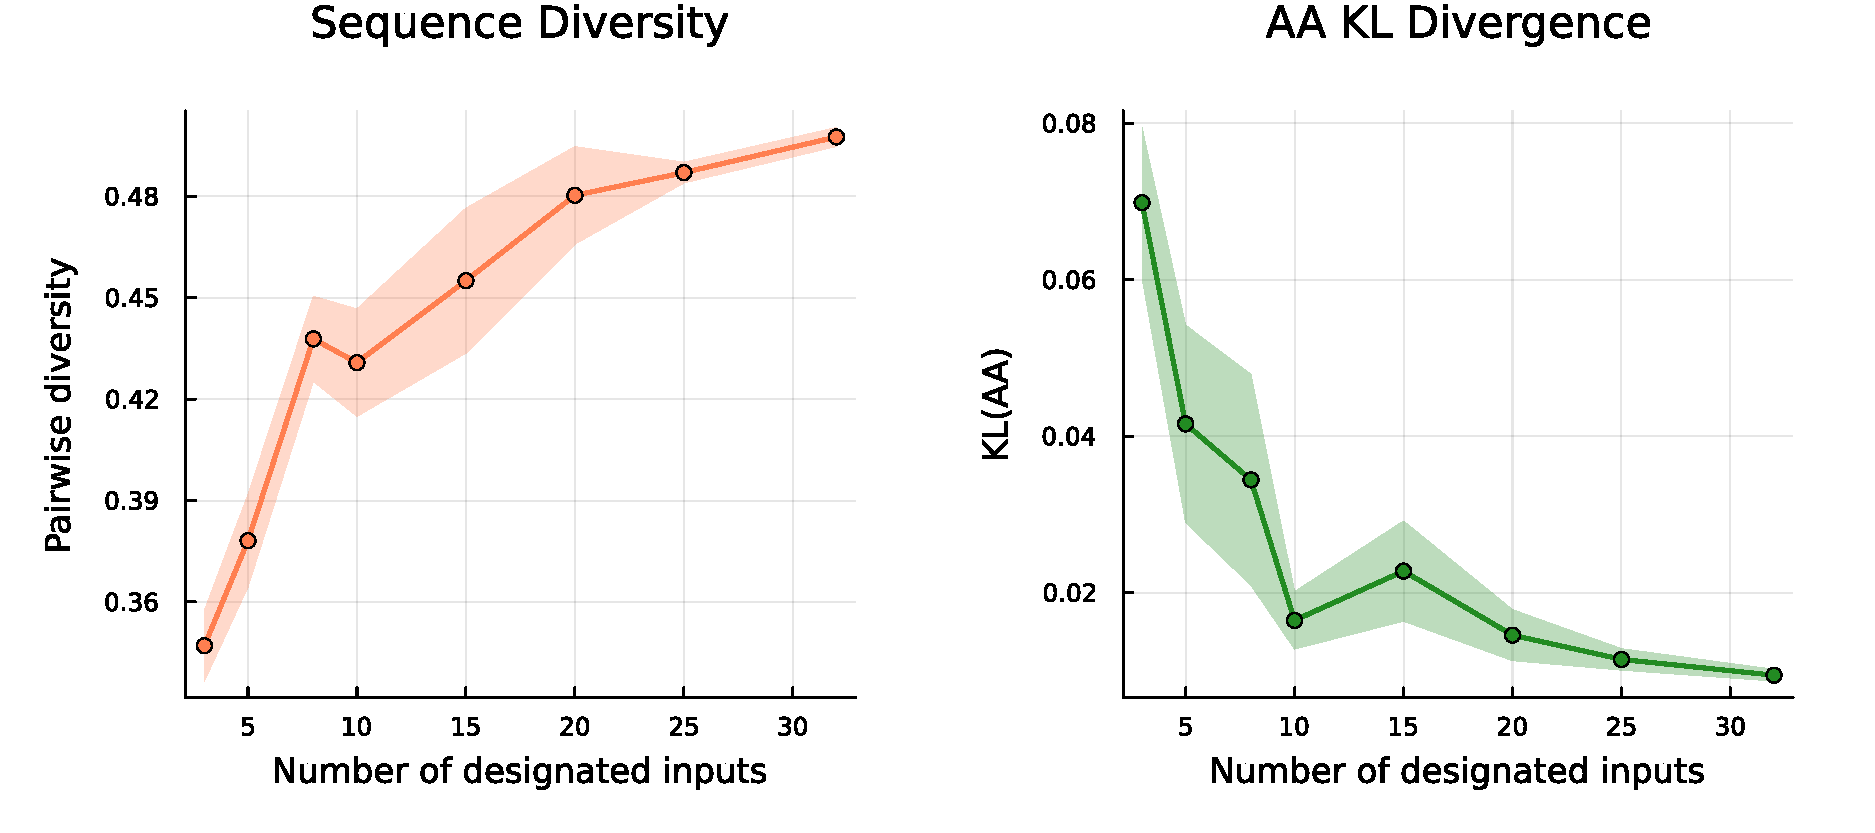
\includegraphics[width=\textwidth]{sections/figs/study1_binder_scaling.pdf}
  \caption{\textbf{Diversity and composition fidelity improve with more input
  K/R-positive sequences; marker retention is complete at every sample size.}
  Subsampling $K_{\mathrm{des}} \in \{3,5,8,10,15,20,25,32\}$ sequences from
  the Kunitz K/R-positive set (3 replicates each; shaded bands show $\pm 1$
  s.d.). P1 K/R fraction was 1.0 at every sample size (not shown).
  \textit{Left:} Pairwise sequence diversity increases from 0.36
  ($K_{\mathrm{des}}=3$) to 0.50 ($K_{\mathrm{des}}=32$).
  \textit{Right:} KL divergence of amino acid composition decreases from 0.047
  to 0.009 over the same range. Three input binders suffice for perfect
  K/R marker retention; more inputs improve the compositional and diversity
  quality of the generated library.}
  \label{fig:scaling}
\end{figure}

% -----------------------------------------------------------------------
% Fig 2: Phase transition entropy curves (old rho sweep figure removed)
% -----------------------------------------------------------------------
\begin{figure}[p]
  \centering
  
\includegraphics[width=0.82\textwidth]{sections/figs/fig5_entropy_curves.pdf}
  \caption{\textbf{Phase transition shifts rightward with increasing multiplicity
  ratio $\rho$.}
  Attention entropy $H(\beta)$ normalized by $\log K$ (the uniform limit) as a
  function of inverse temperature $\beta$ (log scale) for
  $\rho \in \{1, 5, 20, 100, 1000\}$ on the Kunitz family ($K=99$,
  $K_{\mathrm{des}}=32$). At $\rho=1$ (standard SA), the entropy starts at
  $H/\log K = 1$ (uniform attention over all patterns); as $\rho$ increases,
  the multiplicity bias pre-concentrates the attention distribution, lowering the
  starting entropy toward $\log K_{\mathrm{des}} / \log K \approx 0.75$ (dotted
  line). Each curve shows a sigmoidal drop to near-zero entropy (retrieval phase);
  dots and dashed vertical lines mark the inflection point $\beta^{*}(\rho)$.
  As $\rho$ increases from 1 to 1000, $K_{\mathrm{eff}}$ decreases from 99 to
  32.1 and $\beta^{*}$ shifts rightward from 4.4 to 9.3, consistent with fewer
  effective attractors requiring higher inverse temperature to produce an ordered
  phase.}
  \label{fig:phase-transition}
\end{figure}

% -----------------------------------------------------------------------
% Fig 3: Separation index vs. calibration gap
% -----------------------------------------------------------------------
\begin{figure}[p]
  \centering
  
\includegraphics[width=\textwidth]{sections/figs/fig2_separation_vs_gap.pdf}
  \caption{\textbf{Calibration trajectories reveal family-dependent gaps associated with
  PCA-space separation.}
  \textbf{(A)}~Observed marker fraction $f_{\mathrm{obs}}$ versus effective designated
  fraction $f_{\mathrm{eff}}$ as the multiplicity ratio $\rho$ increases from 1 to 500
  for six protein families. The dashed diagonal marks perfect calibration
  ($f_{\mathrm{obs}} = f_{\mathrm{eff}}$). Homeobox
  ($S = \HomeoboxSeparation$) and SH3 ($S = \SHThreeSeparation$)
  domains track the diagonal closely; Kunitz ($S = \KunitzSeparation$) and Forkhead
  ($S = \ForkheadSeparation$) curve below; WW domains ($S = \WWSeparation$) show the
  largest departure; $\omega$-conotoxin ($S = \ConotoxinSeparation$) shows a moderate gap
  despite high PCA separation. Double-headed arrows
  indicate the calibration gap at $\rho = 500$.
  \textbf{(B)}~Fisher separation index $S$ versus calibration gap $\Delta$ at $\rho = 500$.
  Error bars show replicate s.d. An exploratory linear fit to the five Pfam families
  (filled markers; $\Delta \approx \RelationIntercept{} \RelationSlope\,S$,
  $R^{2}=\RelationRsq$) summarizes the association without defining a prospective
  threshold. The $\omega$-conotoxin point (open diamond) is displayed as an external
  comparison and is not included in the fit.}
  \label{fig:separation-vs-gap}
\end{figure}

% -----------------------------------------------------------------------
% Fig: Hard-mask beta sweep (rho -> infinity endpoint)
% -----------------------------------------------------------------------
\begin{figure}[t]
  \centering
  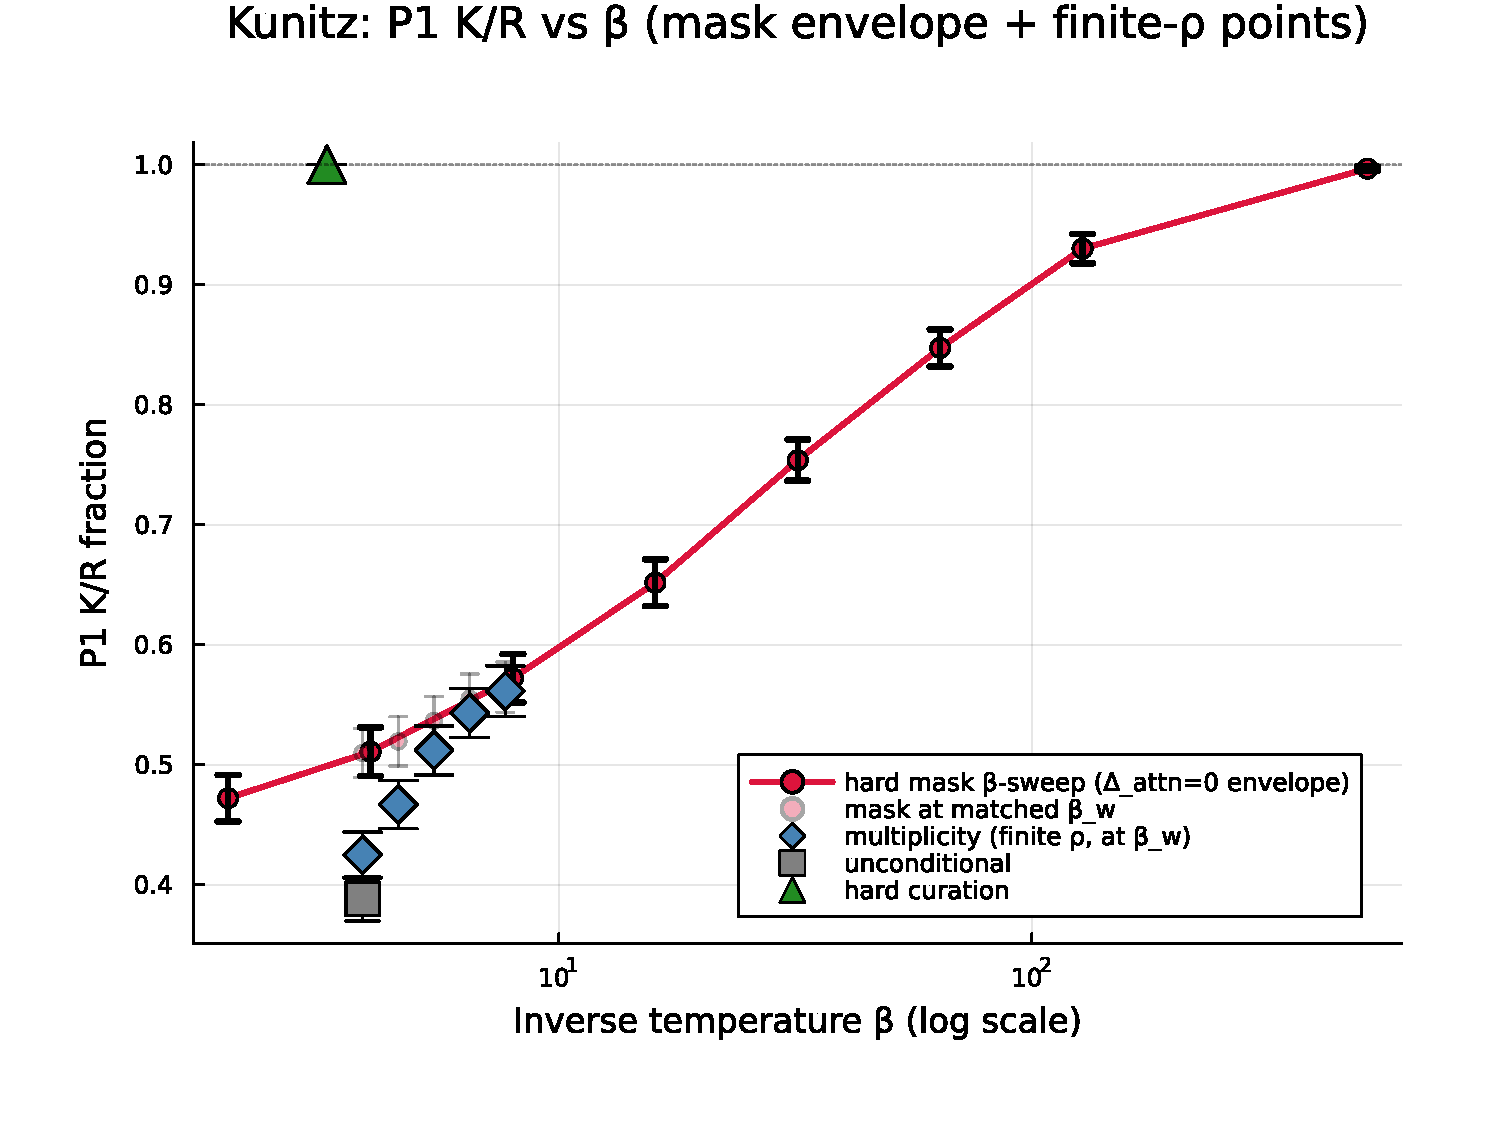
\includegraphics[width=0.72\textwidth]{sections/figs/fig_mask_betasweep.pdf}
  \caption{\textbf{Recovery is set by retrieval sharpness and conditioning strength, both
  acting through the decode gap.}
  P1~K/R fraction for the Kunitz designated subset versus inverse temperature
  $\beta$ (log scale) under the hard attention mask ($b = -\infty$ on background
  patterns; red curve, 30 chains per point, error bars are standard error across
  chains). The mask is the $\Delta_{\mathrm{attn}} = 0$ envelope: recovery climbs
  monotonically from 0.46 at $\beta = 2$ to 1.00 at $\beta = 512$ with no plateau.
  The finite-$\rho$ multiplicity conditions (blue diamonds, each at its own
  $\beta^{*}(\vr)$) sit below this envelope at matched $\beta$: hard masking recovers more
  marker signal than soft weighting by 0.111 (SE 0.027) at $f_{\mathrm{eff}} = 0.5$,
  contracting into the noise as $\rho \to \infty$ (0.002, SE 0.030, at
  $f_{\mathrm{eff}} = 0.99$); faint red points show the mask run at each matched
  $\beta$. Since $\Delta_{\mathrm{attn}} \approx 0$ (attention tracks $f_{\mathrm{eff}}$), this
  is a decode effect, not an attention effect. Hard curation (green triangle) reaches complete transfer at low $\beta$ on
  its subset-only basis; unconditional generation (gray square) is shown for
  reference.}
  \label{fig:mask-betasweep}
\end{figure}

% -----------------------------------------------------------------------
% Table: Hard-mask recovery across the conditioning axis
% -----------------------------------------------------------------------
\begin{table}[t]
  \centering
  \caption{\textbf{Kunitz P1~K/R recovery across the conditioning axis.} Designated
  subset is K/R at the P1 position ($K_{\mathrm{des}} = 32$). All conditions use the
  full-family PCA basis except hard curation, which rebuilds the basis from the
  designated subset. The hard mask ($b = -\infty$ on background) is the
  $\rho \to \infty$ endpoint of the multiplicity axis at fixed $\beta$. Novelty is one
  minus the mean nearest-neighbor identity to the training alignment. P1~K/R is the chain-level
  mean $\pm$ standard error over 30 chains; novelty standard errors are below 0.01.}
  \label{tab:mask-recovery}
  \begin{tabular}{@{}lccc@{}}
    \toprule
    Condition & $\beta$ & P1~K/R $\uparrow$ & Novelty \\
    \midrule
    Unconditional ($b = 0$)                      & 3.8 & $0.39 \pm 0.02$ & 0.42 \\
    Multiplicity (strongest finite $\rho$)       & 7.7 & $0.59 \pm 0.02$ & 0.39 \\
    Hard mask ($b = -\infty$), at $\beta^{*}$    & 3.2 & $0.50 \pm 0.02$ & 0.42 \\
    Hard mask ($b = -\infty$), $\beta = 512$     & 512 & $1.00 \pm 0.00$ & 0.16 \\
    Hard curation (subset basis)                 & 3.2 & $1.00 \pm 0.00$ & 0.32 \\
    \bottomrule
  \end{tabular}
\end{table}

% -----------------------------------------------------------------------
% Table: Per-family rho sweep (replaces old Fig 7)
% -----------------------------------------------------------------------
\begin{table}[p]
  \centering
  \caption{\textbf{Per-family $\rho$ sweep: mean attention weights track
  $f_{\mathrm{eff}}$ closely; decoded marker fidelity varies across PCA
  geometries.} Selected $\rho$ values for each family.
  $f_{\mathrm{eff}}$: effective designated fraction from multiplicity weights;
  $\bar{a}_{\mathrm{des}}$: mean softmax attention on designated patterns;
  $f_{\mathrm{obs}}$: mean hard-decoded marker fraction across five independent
  replicates (620 retained samples per replicate); error bars are replicate s.d.;
  $D$: mean pairwise diversity.
  In all families $\bar{a}_{\mathrm{des}} \approx f_{\mathrm{eff}}$
  within finite-sample uncertainty, but $f_{\mathrm{obs}}$ converges fastest
  for Homeobox ($S=\HomeoboxSeparation$) and slowest for WW
  ($S=\WWSeparation$), reflecting the
  observed latent-to-sequence calibration gap.}
  \label{tab:per-family-rho}
  \small
  \resizebox{\textwidth}{!}{%
  \begin{tabular}{llcccccc}
    \toprule
    Family & ($K$, $K_{\mathrm{des}}$, $S$)
      & $\rho$ & $f_{\mathrm{eff}}$ & $\bar{a}_{\mathrm{des}}$
      & $f_{\mathrm{obs}}$ & $\Delta$ & $D$ \\
    \midrule
    \multirow{4}{*}{WW} & \multirow{4}{*}{(420, 69, 0.11)} & 1 & 0.164 & $0.166 \pm 0.003$ & $0.138 \pm 0.006$ & 0.03 & 0.690 \\
& & 10 & 0.663 & $0.656 \pm 0.003$ & $0.210 \pm 0.003$ & 0.45 & 0.668 \\
& & 100 & 0.952 & $0.953 \pm 0.001$ & $0.275 \pm 0.009$ & 0.68 & 0.648 \\
& & 500 & 0.990 & $0.990 \pm 0.000$ & $0.332 \pm 0.004$ & 0.66 & 0.637 \\
\midrule
\multirow{4}{*}{Forkhead} & \multirow{4}{*}{(246, 122, 0.17)} & 1 & 0.496 & $0.477 \pm 0.003$ & $0.544 \pm 0.004$ & -0.05 & 0.484 \\
& & 10 & 0.908 & $0.904 \pm 0.001$ & $0.630 \pm 0.003$ & 0.28 & 0.461 \\
& & 100 & 0.990 & $0.991 \pm 0.000$ & $0.729 \pm 0.004$ & 0.26 & 0.416 \\
& & 500 & 0.998 & $0.998 \pm 0.000$ & $0.759 \pm 0.007$ & 0.24 & 0.399 \\
\midrule
\multirow{4}{*}{Kunitz} & \multirow{4}{*}{(99, 32, 0.20)} & 1 & 0.323 & $0.311 \pm 0.003$ & $0.366 \pm 0.006$ & -0.04 & 0.556 \\
& & 10 & 0.827 & $0.811 \pm 0.002$ & $0.492 \pm 0.007$ & 0.33 & 0.537 \\
& & 100 & 0.979 & $0.975 \pm 0.001$ & $0.535 \pm 0.011$ & 0.44 & 0.520 \\
& & 500 & 0.996 & $0.994 \pm 0.000$ & $0.579 \pm 0.006$ & 0.42 & 0.509 \\
\midrule
\multirow{4}{*}{SH3} & \multirow{4}{*}{(55, 33, 0.34)} & 1 & 0.600 & $0.615 \pm 0.004$ & $0.825 \pm 0.003$ & -0.22 & 0.582 \\
& & 10 & 0.938 & $0.939 \pm 0.001$ & $0.887 \pm 0.003$ & 0.05 & 0.582 \\
& & 100 & 0.993 & $0.993 \pm 0.000$ & $0.988 \pm 0.001$ & 0.01 & 0.530 \\
& & 500 & 0.999 & $0.998 \pm 0.000$ & $0.992 \pm 0.001$ & 0.01 & 0.510 \\
\midrule
\multirow{4}{*}{Homeobox} & \multirow{4}{*}{(136, 102, 0.42)} & 1 & 0.750 & $0.770 \pm 0.003$ & $0.933 \pm 0.004$ & -0.18 & 0.523 \\
& & 10 & 0.968 & $0.966 \pm 0.001$ & $0.931 \pm 0.005$ & 0.04 & 0.515 \\
& & 100 & 0.997 & $0.997 \pm 0.000$ & $0.914 \pm 0.007$ & 0.08 & 0.531 \\
& & 500 & 0.999 & $0.999 \pm 0.000$ & $0.920 \pm 0.004$ & 0.08 & 0.534 \\
\midrule
\multirow{4}{*}{$\omega$-Conotoxin} & \multirow{4}{*}{(74, 23, 0.78)} & 1 & 0.311 & $0.334 \pm 0.006$ & $0.492 \pm 0.007$ & -0.18 & 0.563 \\
& & 10 & 0.819 & $0.826 \pm 0.003$ & $0.684 \pm 0.009$ & 0.13 & 0.509 \\
& & 100 & 0.978 & $0.979 \pm 0.002$ & $0.828 \pm 0.008$ & 0.15 & 0.446 \\
& & 500 & 0.996 & $0.995 \pm 0.000$ & $0.874 \pm 0.012$ & 0.12 & 0.433 \\
\bottomrule

  \end{tabular}
  }
\end{table}

% -----------------------------------------------------------------------
% Table 2: Merged validation + baseline comparison
% -----------------------------------------------------------------------
\begin{table}[p]
  \centering
  \caption{\textbf{Structure-model, language-model, and sequence-marker evaluation on the Kunitz domain.}
  pLDDT: ESMFold predicted confidence (0--100; $>70$ = confident).
  TM: TM-score against 1BPI chain~A ($>0.5$ = same fold).
  PPL: ESM2-650M masked-marginal pseudo-perplexity (lower = more plausible).
  P1~K/R: fraction with Lys/Arg at the primary trypsin contact.
  KL: amino acid composition divergence ($\times 10^{3}$).
  $D$: mean pairwise diversity.
  Structural and LM values are mean $\pm$ s.d.\ across 50 sequences;
  sequence-level metrics are mean $\pm$ s.d.\ across 5 replicates.
  SA-generated and stored sequences have similar structure-model and language-model
  summaries. Conditioning on the K/R-positive subset yields complete K/R marker retention;
  this is not an experimental binding measurement.}
  \label{tab:structure-validation}
  \small
  \resizebox{\textwidth}{!}{%
  \begin{tabular}{lcccccc}
    \toprule
    Source & pLDDT & TM & PPL & P1 K/R & KL ($\times 10^{3}$) & $D$ \\
    \midrule
    Stored (natural)      & $89.3 \pm 3.2$  & $0.83 \pm 0.03$ & $4.97 \pm 0.98$ & 0.32 & 0 & 0.63 \\
    SA (full family)      & $90.4 \pm 1.2$  & $0.84 \pm 0.01$ & $4.78 \pm 0.64$ & $0.41 \pm 0.01$ & $6.9 \pm 0.1$ & 0.56 \\
    SA (K/R-positive)     & $90.7 \pm 1.1$  & $0.83 \pm 0.01$ & $4.72 \pm 0.60$ & $1.00 \pm 0.00$ & $19.5 \pm 0.4$ & 0.50 \\
    SA (K/R-negative)     & $91.0 \pm 1.2$  & $0.85 \pm 0.01$ & $4.73 \pm 0.72$ & $0.00 \pm 0.00$ & $12.4 \pm 0.3$ & 0.53 \\
    HMM emit (HMMER3)     & $60.4 \pm 13.1$ & $0.60 \pm 0.19$ & $16.1 \pm 4.2$  & $0.15 \pm 0.03$ & $29.7 \pm 11.3$ & 0.56 \\
    Bootstrap (resample)  & ---             & ---              & ---              & $0.30 \pm 0.04$ & $1.0 \pm 0.3$ & 0.56 \\
    \bottomrule
  \end{tabular}
  }
\end{table}

% -----------------------------------------------------------------------
% Table: AF2 cross-validation
% -----------------------------------------------------------------------
\begin{table}[p]
  \centering
  \caption{\textbf{AlphaFold2-ptm structure-model comparison.}
  Independent structure predictions via ColabFold (AlphaFold2-ptm, 1 model,
  3 recycles, MMseqs2 MSA) for 50 sequences per source.
  pLDDT: mean predicted confidence ($0$--$100$).
  TM: TM-score against experimental reference (1BPI chain~A for Kunitz,
  1OMG chain~A for $\omega$-conotoxin).
  The group summaries are consistent with the ESMFold comparison. They are
  model-derived quantities and do not establish experimental folding or binding.}
  \label{tab:af2-validation}
  \small
  \begin{tabular}{llcccc}
    \toprule
    Family & Source & $n$ & pLDDT & TM-score \\
    \midrule
    \multirow{3}{*}{Kunitz}
      & Stored (natural)       & 50 & $93.5 \pm 4.0$ & $0.83 \pm 0.03$ \\
      & SA (K/R-positive)      & 50 & $94.6 \pm 1.4$ & $0.84 \pm 0.01$ \\
      & SA (full family)       & 50 & $95.0 \pm 1.3$ & $0.85 \pm 0.01$ \\
    \midrule
    \multirow{3}{*}{$\omega$-Conotoxin}
      & Stored (natural)       & 50 & $67.9 \pm 9.8$ & $0.35 \pm 0.11$ \\
      & SA (designated subset) & 50 & $78.5 \pm 4.1$ & $0.47 \pm 0.02$ \\
      & SA (full family)       & 50 & $73.9 \pm 10.4$ & $0.39 \pm 0.12$ \\
    \bottomrule
  \end{tabular}
\end{table}

% -----------------------------------------------------------------------
% Table: ω-Conotoxin pharmacophore inheritance
% -----------------------------------------------------------------------
\begin{table}[p]
  \centering
  \caption{\textbf{$\omega$-Conotoxin Tyr13 marker retention under curated vs.\
  full-family seeding.}
  Tyr13\%: fraction with tyrosine at the selected marker position (col.~13).
  K+R\%: basic residue fraction (electrostatic complementarity). KL: amino acid composition
  divergence. Novelty: mean cosine distance to nearest stored pattern. Designated-subset seeding
  amplifies Tyr13 from 82.6\% to 98.3\% and preserves the basic-residue signature exactly,
  while full-family seeding dilutes both signals.}
  \label{tab:conotoxin-pharmacophore}
  \small
  \begin{tabular}{lccccc}
    \toprule
    Condition & $N$ & Tyr13 (\%) & K+R (\%) & KL & Novelty \\
    \midrule
    Input: full family          &   74 & 33.8 &  9.9 & 0      & 0 \\
    Input: designated subset    &   23 & 82.6 & 19.7 & 0      & 0 \\
    Generated: full-seeded      & 1550 & 46.9 & 12.0 & 0.0075 & 0.60 \\
    Generated: designated-seeded & 1550 & 98.3 & 20.1 & 0.0083 & 0.46 \\
    \bottomrule
  \end{tabular}
\end{table}

% -----------------------------------------------------------------------
% Table: SAR agreement
% -----------------------------------------------------------------------
\begin{table}[ht]
  \caption{\textbf{Residue frequencies at reported $\omega$-conotoxin SAR positions.}
  Published structure--activity relationship (SAR) data for $\omega$-conotoxin
  binding to Cav2.2 identify critical residues whose mutation abolishes or
  substantially reduces channel block~\cite{kimTyr13Essential1995,satoBasicResidues1993,satoAlaScanMVIIC2000,schroederLys2Effects2012,lewisConotoxinSAR2012,schroederChiralityTyr131999}.
  For each reported position, the table gives the fraction retaining the listed residue
  (or a K/R substitution at basic positions). Designated-subset generation retains the
  Tyr13 signal and cysteine scaffold and enriches several reported positions. These
  frequencies do not test the effects of mutations in the generated backgrounds.}
  \label{tab:sar-agreement}
  \centering
  \small
  \begin{tabular}{clllccc}
    \toprule
    Pos. & WT & Role & Mutation effect & Input & SA des. & SA full \\
    \midrule
    13 & Tyr & Primary pharmacophore & Ala: abolishes activity & 0.83 & \textbf{0.98} & 0.47 \\
    2  & Lys & Loop 2 stabilization  & Ala: 40$\times$ loss (GVIA) & 0.96 & \textbf{0.98} & 0.46 \\
    10 & Arg & Loop 2 binding        & Critical for interaction & 0.70 & \textbf{0.82} & 0.35 \\
    11 & Leu & Loop 2 binding        & Critical for interaction & 0.17 & 0.24 & 0.11 \\
    1  & Cys & Disulfide framework   & Required for fold & 1.00 & \textbf{1.00} & 1.00 \\
    8  & Cys & Disulfide framework   & Required for fold & 1.00 & \textbf{1.00} & 1.00 \\
    15 & Cys & Disulfide framework   & Required for fold & 1.00 & \textbf{0.97} & 1.00 \\
    16 & Cys & Disulfide framework   & Required for fold & 0.87 & \textbf{1.00} & 1.00 \\
    20 & Cys & Disulfide framework   & Required for fold & 0.70 & \textbf{1.00} & 1.00 \\
    25 & Cys & Disulfide framework   & Required for fold & 0.52 & \textbf{1.00} & 1.00 \\
    21 & Arg & Electrostatic          & Ala: reduced potency & 0.44 & \textbf{0.66} & 0.14 \\
    4  & Lys & P/Q selectivity       & Ala: important for P/Q & 0.52 & \textbf{0.61} & 0.28 \\
    \bottomrule
  \end{tabular}
\end{table}

% -----------------------------------------------------------------------
% Table: Docking validation
% -----------------------------------------------------------------------
\begin{table}[ht]
\centering
\footnotesize
\setlength{\tabcolsep}{3.5pt}
\caption{\textbf{Low-confidence AlphaFold2-multimer predictions for generated and control
$\omega$-conotoxins.}
Complex-level scores for sequences modeled with the Cav2.2 pore domain via ColabFold in
multimer mode. For each group we report mean values and standard deviations of pTM, iPTM, and
interface pLDDT. The uniformly low absolute values do not establish binding geometry.}
\label{tab:docking-validation}
\begin{tabular}{lcccc}
\toprule
\textbf{Group} & \textbf{n} & \textbf{Mean pTM} & \textbf{Mean iPTM} & \textbf{Mean Interface pLDDT} \\
\midrule
SA designated-subset & 10 & $0.221\pm0.007$ & $0.105\pm0.008$ & $37.2\pm5.4$ \\
SA full-family & 10 & $0.219\pm0.008$ & $0.104\pm0.007$ & $38.2\pm4.0$ \\
Natural controls & 5 & $0.228\pm0.004$ & $0.108\pm0.007$ & $40.7\pm3.5$ \\
\bottomrule
\end{tabular}
\end{table}

% -----------------------------------------------------------------------
% Fig: Binding-loop heatmaps with residuals
% -----------------------------------------------------------------------
\begin{figure}[p]
  \centering
  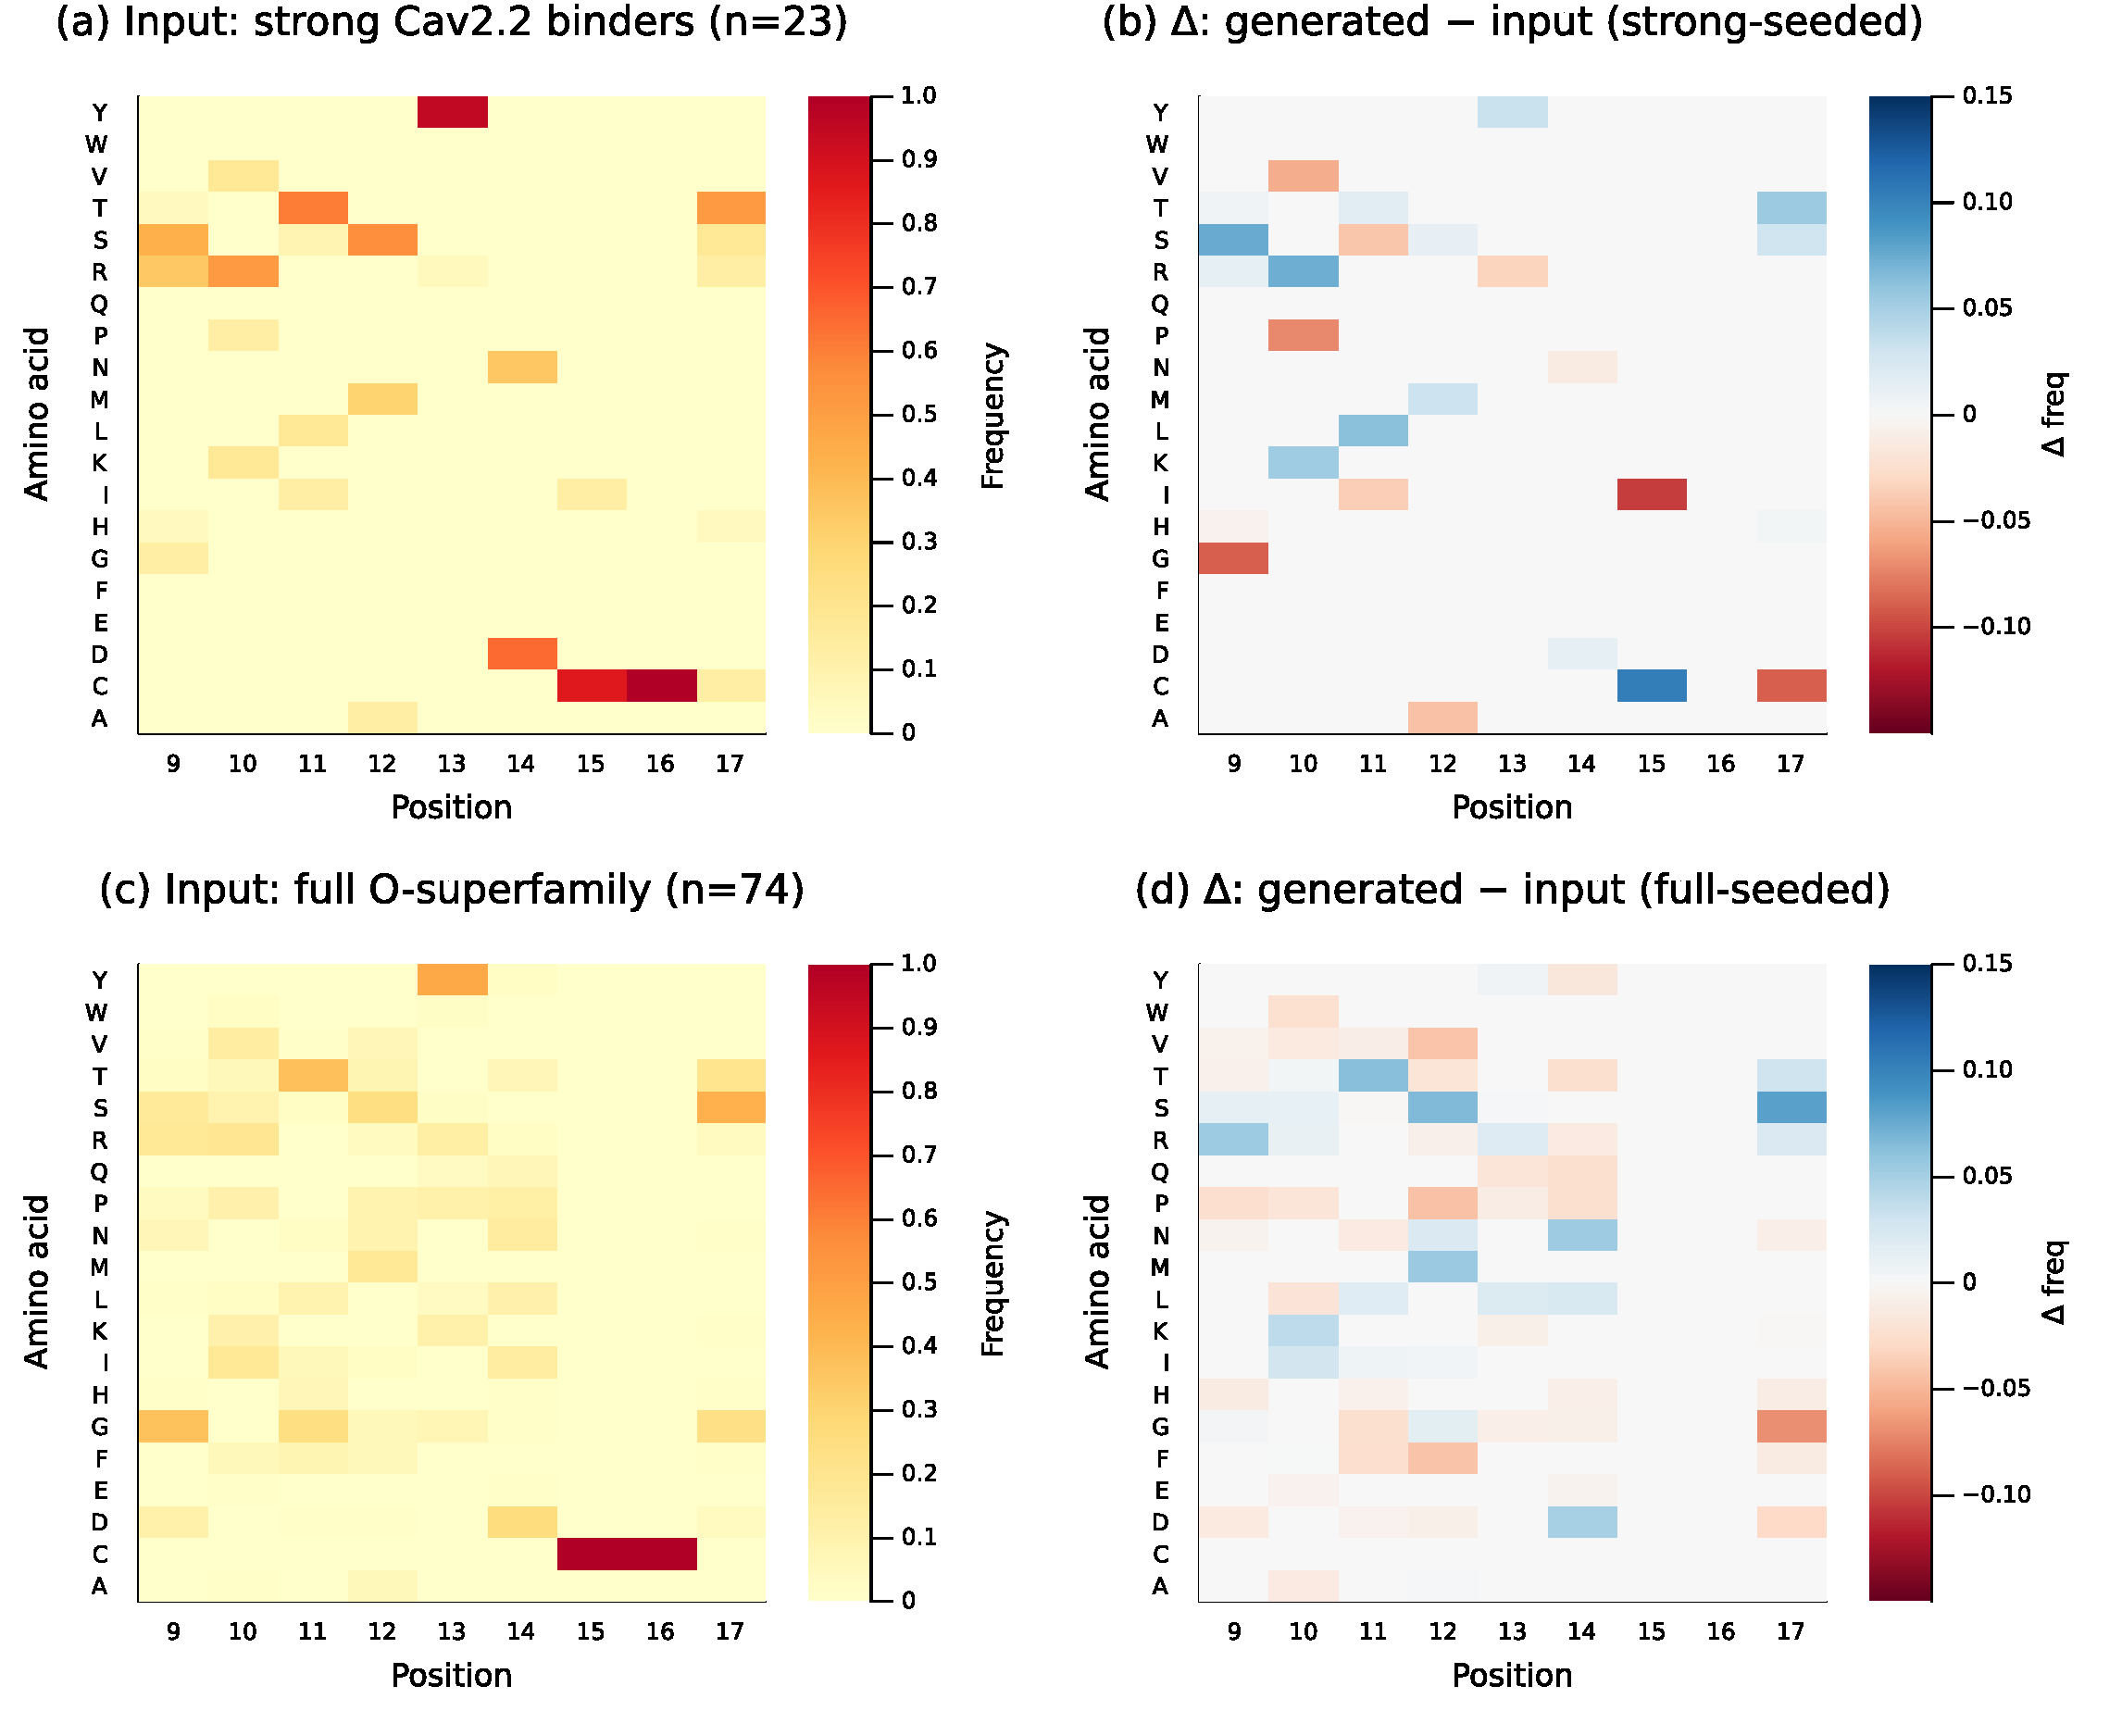
\includegraphics[width=\textwidth]{sections/figs/loop_heatmap_with_residuals.pdf}
  \caption{\textbf{Binding-loop amino acid frequencies and generation residuals for
  the $\omega$-conotoxin family (positions 9--17).}
  \textit{Left column:} Per-position amino acid frequency heatmaps for the input sequences
  (designated subset, $n=23$, panel~a; full O-superfamily, $n=74$, panel~c).
  \textit{Right column:} Residual heatmaps (generated $-$ input) showing the change in
  frequency at each position--residue pair after SA generation. Panel~(b): designated-seeded
  residuals are near-zero throughout ($|\Delta f| < 0.15$), confirming that the Tyr
  pharmacophore at position~13, the conserved Cys framework (positions~14--16), and the
  variable-loop diversity (positions~9--12) are reproduced with high fidelity. Panel~(d):
  full-seeded residuals are slightly larger, reflecting the broader sequence diversity of
  the input. Blue: enrichment; red: depletion; white: no change.}
  \label{fig:conotoxin-loop}
\end{figure}

% -----------------------------------------------------------------------
% Fig: Sequence-level analysis
% -----------------------------------------------------------------------
\begin{figure}[p]
  \centering
  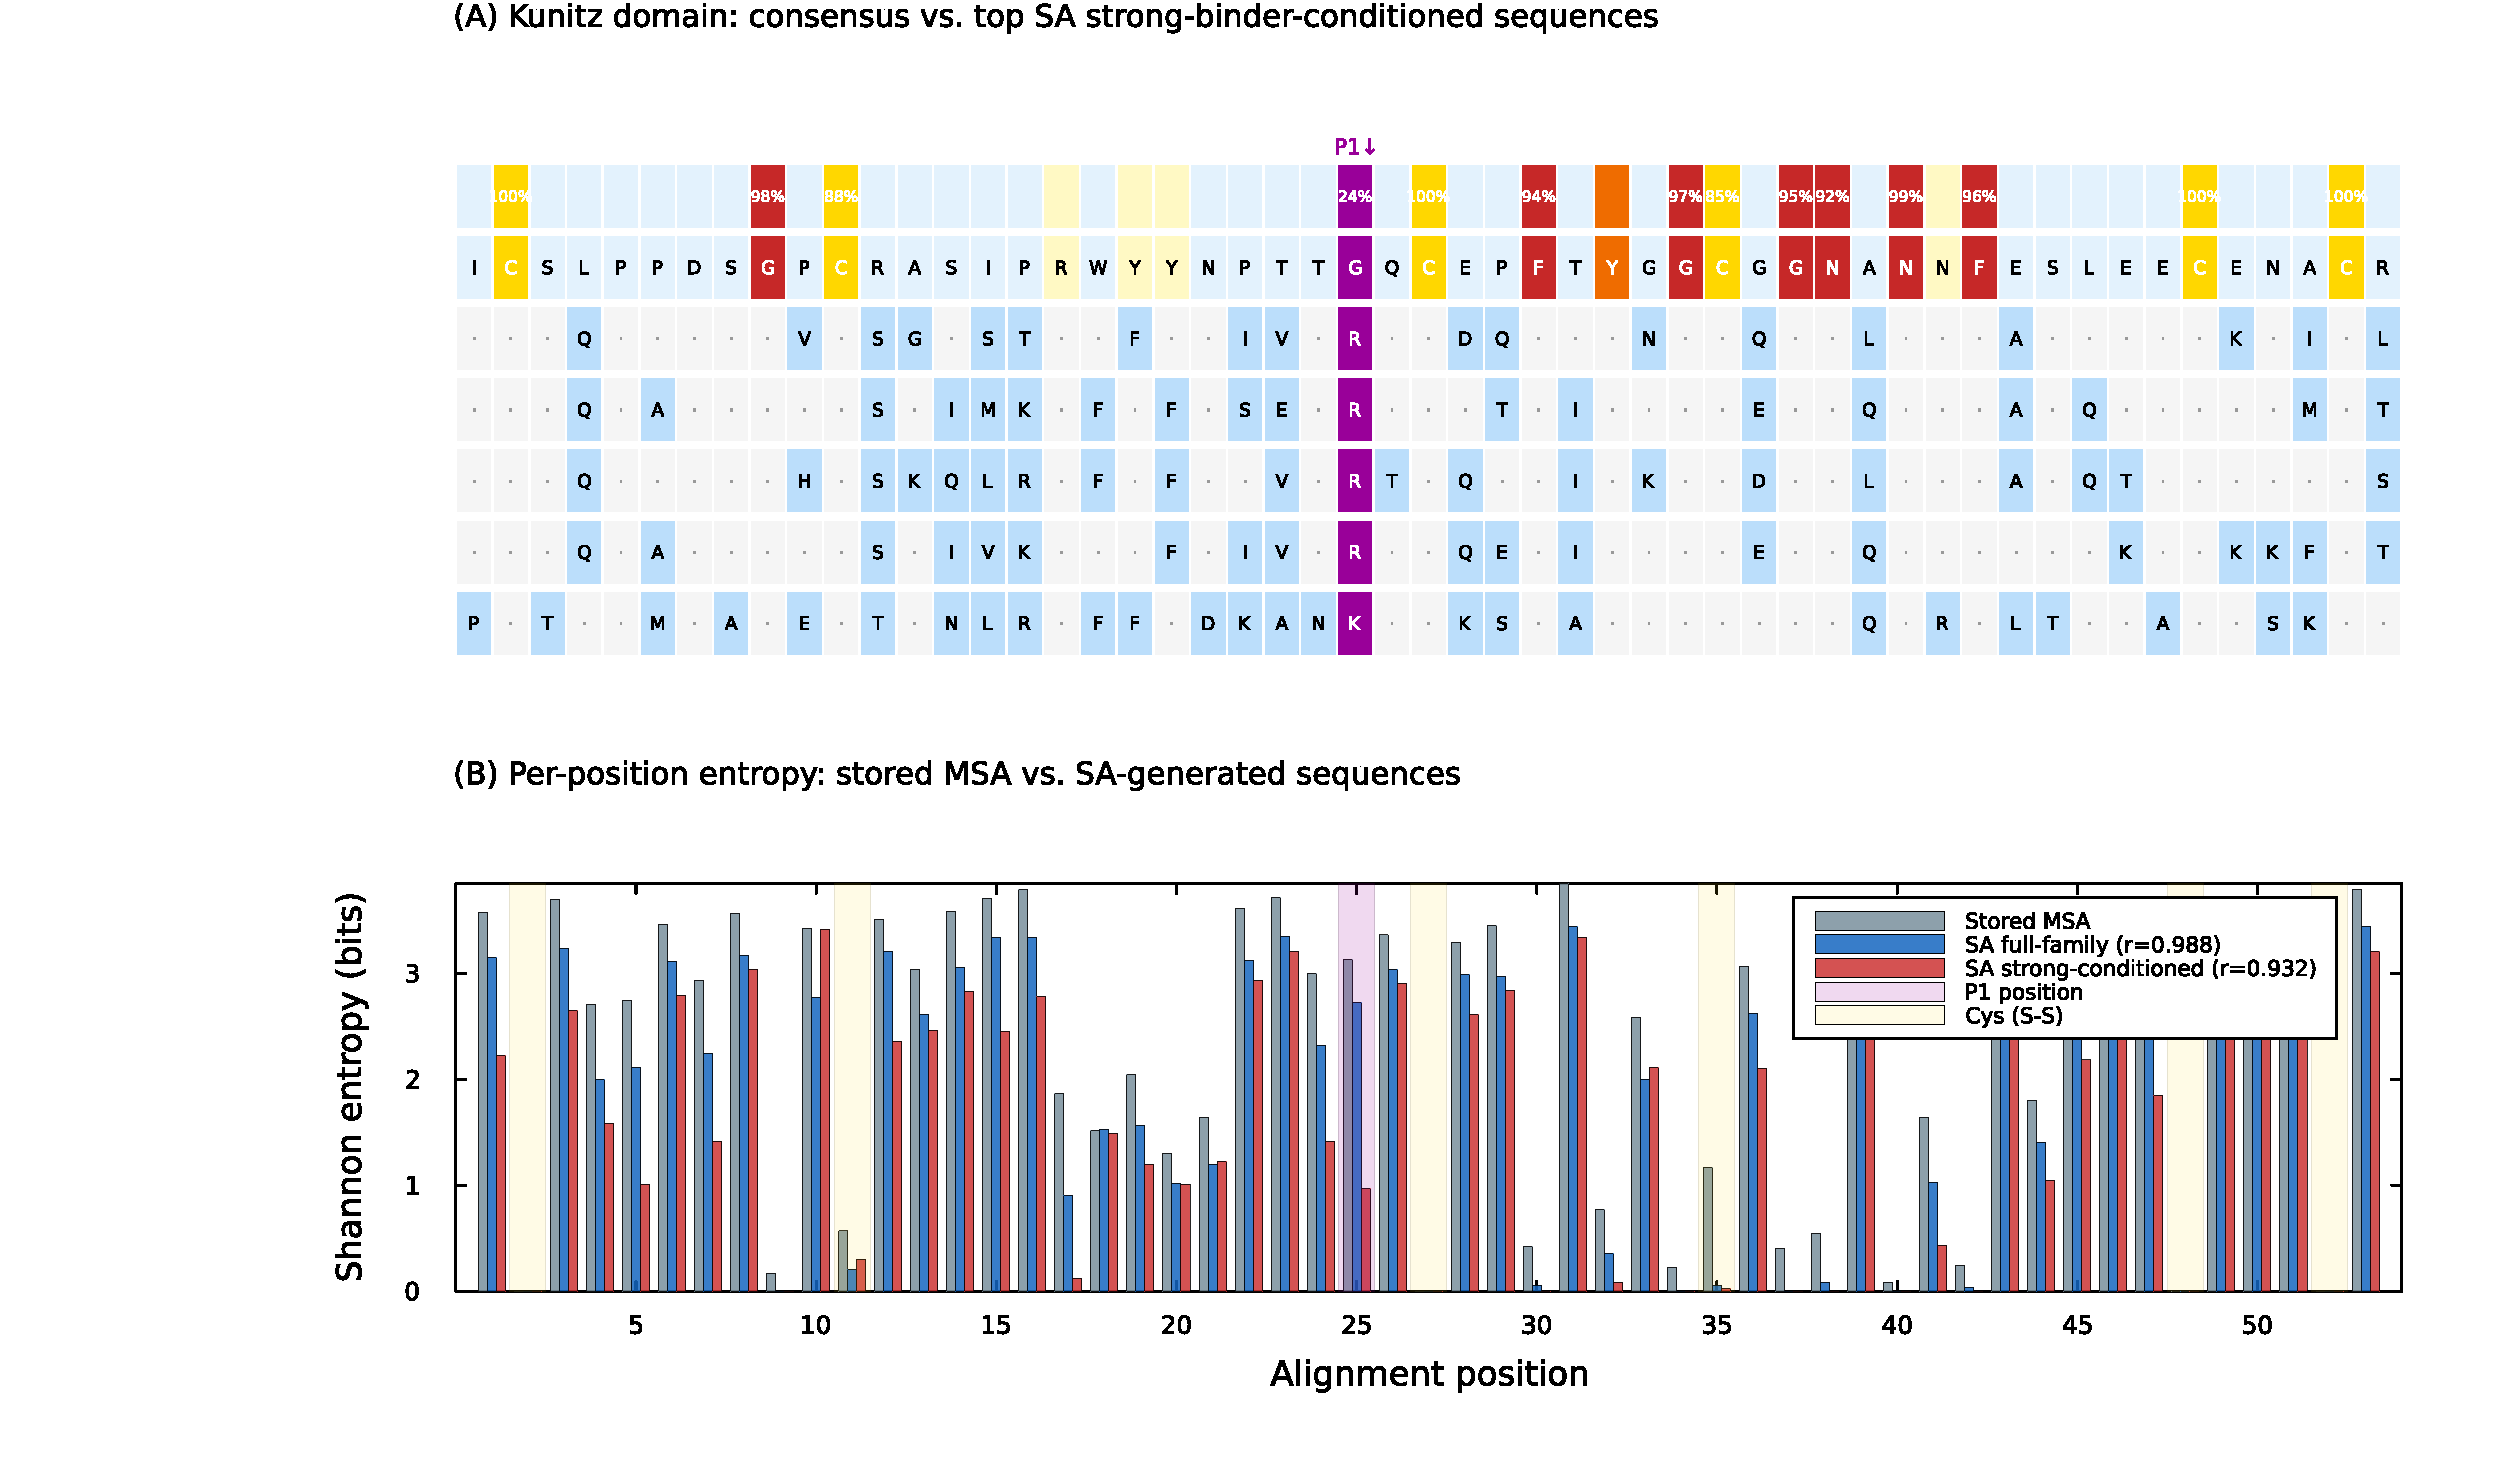
\includegraphics[width=\textwidth]{sections/figs/sequence_analysis_kunitz.pdf}
  \caption{\textbf{Sequence-level analysis of SA-generated Kunitz domain sequences
  conditioned on the K/R-positive subset.}
  \textbf{(A)}~Alignment of the family consensus with the five highest-confidence
  SA K/R-positive-subset-conditioned sequences (ranked by ESMFold pLDDT). Positions are
  colored by conservation in the stored MSA: highly conserved ($>90\%$, red),
  conserved ($70$--$90\%$, orange), moderate ($50$--$70\%$, yellow), and variable
  ($<50\%$, blue). Cysteines forming the three disulfide bonds are highlighted in
  gold; the P1 position is highlighted in purple. Dots indicate matches to the
  consensus; letters indicate substitutions. All five sequences preserve every
  highly conserved position ($11/11$), all six cysteines ($6/6$), and carry K or R
  at P1, while introducing $19$--$26$ substitutions concentrated at variable sites.
  \textbf{(B)}~Per-position Shannon entropy for the stored MSA (gray), SA full-family
  generation (blue), and SA K/R-positive-subset-conditioned generation (red). The
  full-family entropy correlation is very high ($r = 0.988$), confirming that SA
  recapitulates the position-specific conservation pattern of the natural family.
  The K/R-positive-subset correlation is slightly lower ($r = 0.932$), with
  the largest deviation at the P1 position (column~25): conditioning collapses P1
  diversity to K/R, reducing entropy at this site while preserving the entropy
  profile elsewhere.}
  \label{fig:sequence-analysis}
\end{figure}

% -----------------------------------------------------------------------
% Fig: Conotoxin sequence-level analysis
% -----------------------------------------------------------------------
\begin{figure}[p]
  \centering
  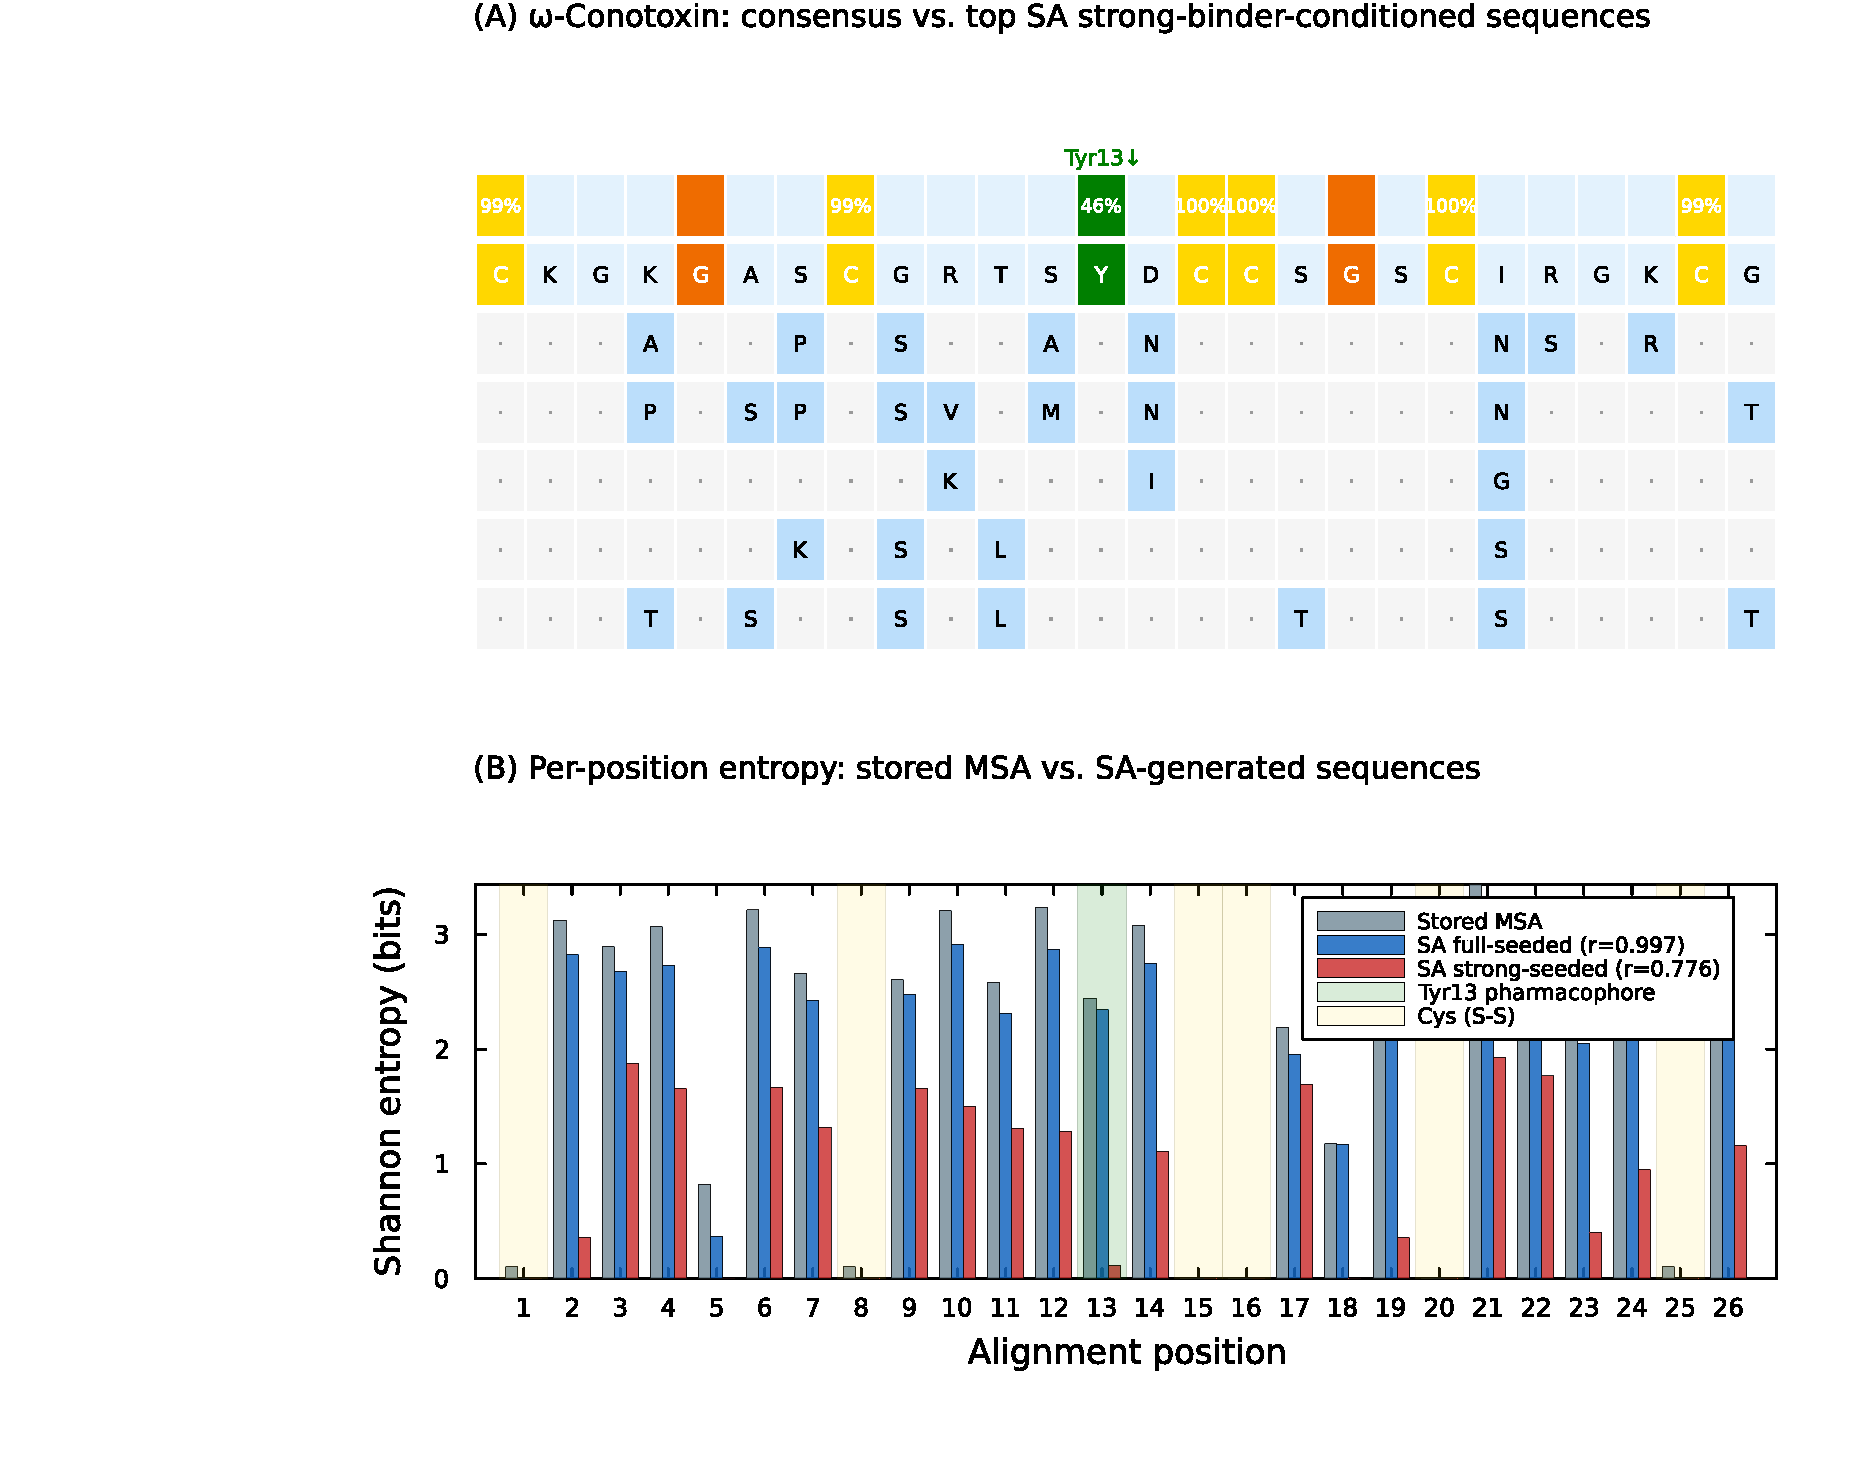
\includegraphics[width=\textwidth]{sections/figs/sequence_analysis_conotoxin.pdf}
  \caption{\textbf{Sequence-level analysis of SA-generated $\omega$-conotoxin sequences
  conditioned on the designated subset.}
  \textbf{(A)}~Alignment of the family consensus with the five highest-confidence
  SA designated-subset-conditioned sequences (ranked by ESMFold pLDDT). Positions are
  colored by conservation in the stored MSA: highly conserved ($>90\%$, red),
  conserved ($70$--$90\%$, orange), moderate ($50$--$70\%$, yellow), and variable
  ($<50\%$, blue). Cysteines forming the three disulfide bonds are highlighted in
  gold; the Tyr13 pharmacophore position is highlighted in green. All five sequences
  preserve every highly conserved position ($6/6$), all six cysteines ($6/6$), and
  carry Tyr at the pharmacophore position, while introducing $5$--$11$ substitutions
  concentrated at variable sites.
  \textbf{(B)}~Per-position Shannon entropy for the stored MSA (gray), SA full-seeded
  generation (blue), and SA designated-seeded generation (red). The full-seeded entropy
  correlation is near-perfect ($r = 0.997$), confirming faithful recapitulation of
  position-specific conservation. The designated-seeded correlation is lower
  ($r = 0.745$), reflecting lower diversity after conditioning on the 23-sequence
  designated subset, including at Tyr13 and co-varying loop residues.}
  \label{fig:conotoxin-sequence-analysis}
\end{figure}

% -----------------------------------------------------------------------
% Fig: Combined fold superposition (Kunitz + Conotoxin)
% -----------------------------------------------------------------------
\begin{figure}[p]
  \centering
  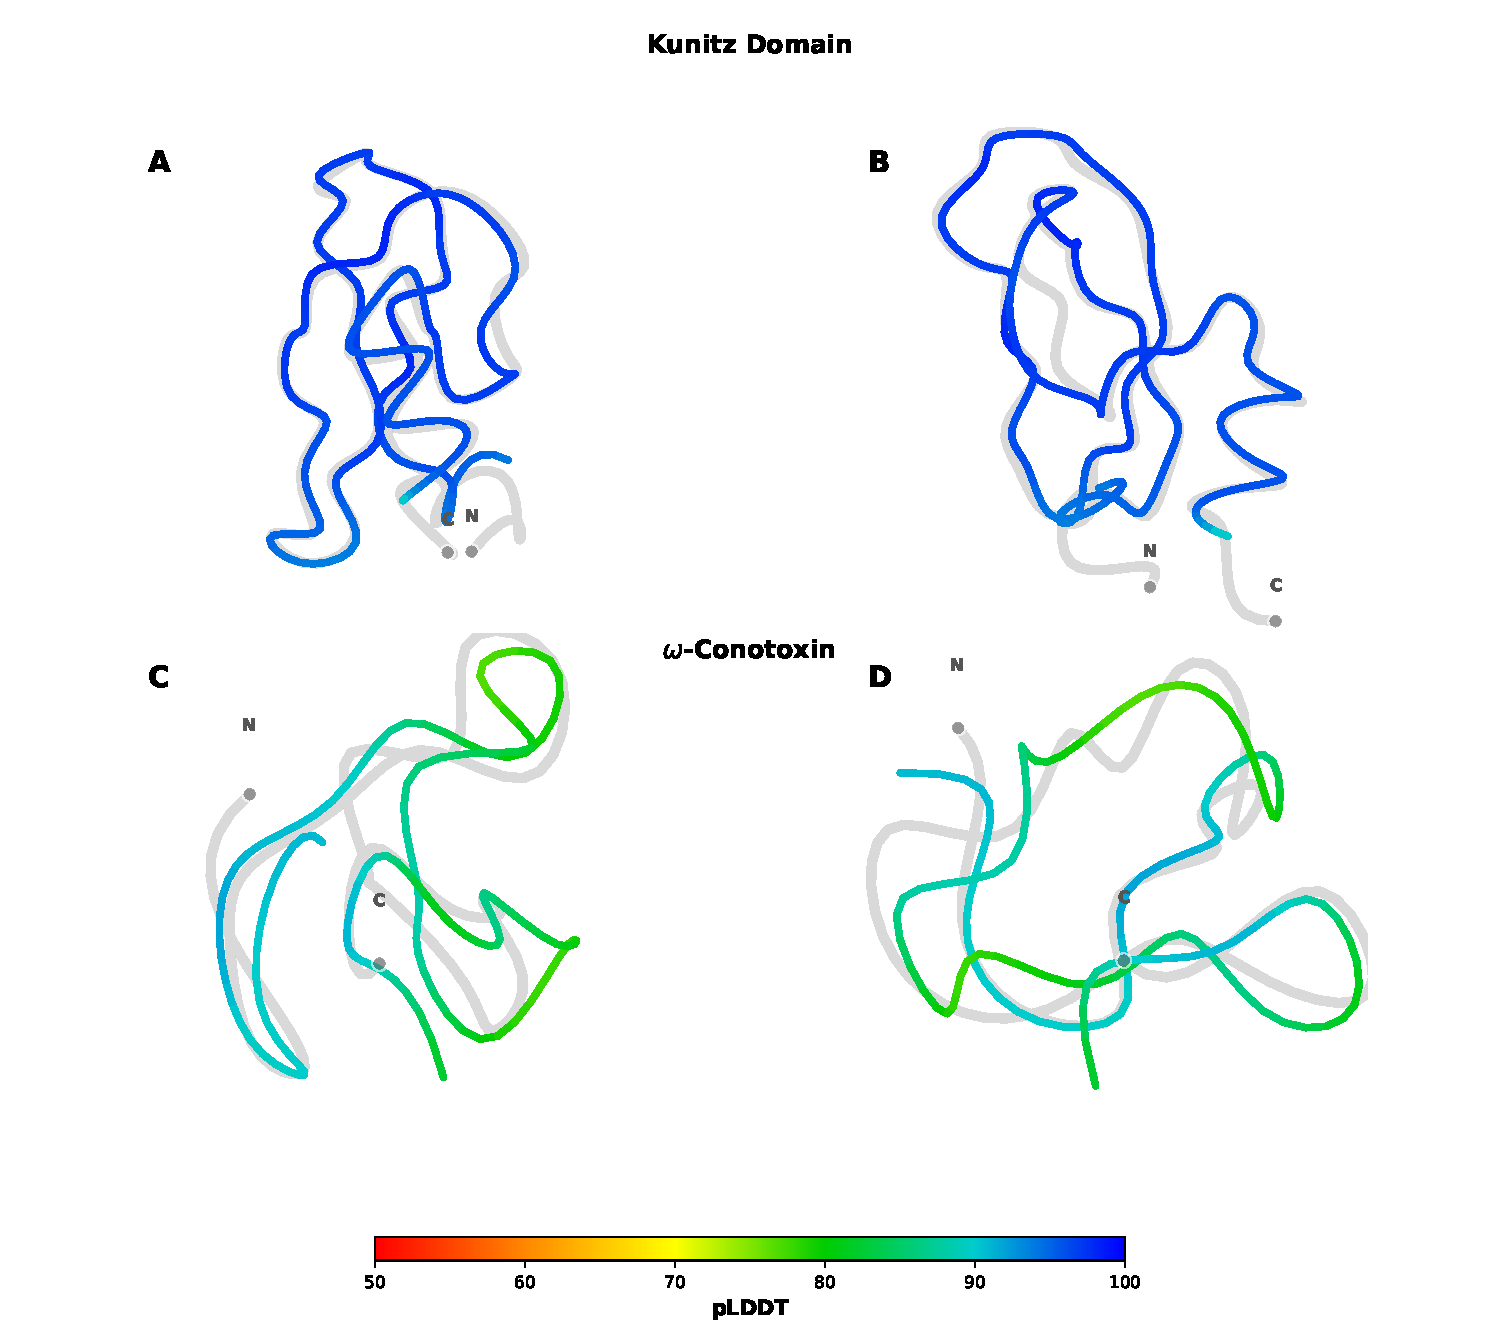
\includegraphics[width=\textwidth]{figs/fold_superposition_combined.pdf}
  \caption{\textbf{Structure models place selected SA-generated sequences near
  experimental family references.}
  For each family, the single highest TM-score SA designated-subset-conditioned sequence
  (colored by per-residue pLDDT confidence) is superimposed onto the experimental
  reference structure (gray, semi-transparent) and shown in two orthogonal views
  (front and $90^{\circ}$ rotation) to reveal the full three-dimensional architecture.
  \textbf{(A)}~Kunitz domain, front view. \textbf{(B)}~Kunitz domain, $90^{\circ}$
  rotation. The SA-generated variant aligns to the BPTI crystal structure
  (1BPI chain~A) with TM $= 0.94$, reproducing the double-loop architecture,
  three-stranded antiparallel $\beta$-sheet, and $\alpha$-helical turn;
  pLDDT $> 90$ throughout (deep blue) indicates high-confidence prediction.
  \textbf{(C)}~$\omega$-Conotoxin, front view. \textbf{(D)}~$\omega$-Conotoxin,
  $90^{\circ}$ rotation. The SA-generated variant aligns to the MVIIA NMR structure
  (1OMG chain~A) with TM $= 0.53$, consistent with the small peptide length
  (26 residues) where TM-score normalization is noisy; the cystine-knot topology
  and loop architecture appear in the prediction, with pLDDT $\sim 80$ (cyan/green).
  Colorbar: pLDDT confidence scale (red $= 50$, blue $= 100$).
  Structures predicted by ESMFold~\cite{esmfold2022}; alignment by
  TM-align~\cite{tmAlign2005}.}
  \label{fig:fold-superposition}
\end{figure}

% --- SI Appendix ---
\clearpage
\setcounter{figure}{0}
\setcounter{table}{0}
\renewcommand{\thefigure}{S\arabic{figure}}
\renewcommand{\thetable}{S\arabic{table}}
\setcounter{section}{0}
\renewcommand{\thesection}{S\arabic{section}}
\renewcommand{\theHfigure}{S\arabic{figure}}
\renewcommand{\theHtable}{S\arabic{table}}
\renewcommand{\theHsection}{S\arabic{section}}

\section*{SI Appendix}
% appendix.tex -- Supplementary Material

\section{Sequence Encoding, PCA Projection, and Multiplicity Conditioning}\label{app:pca}

Stochastic attention (SA) operates on continuous vectors on the unit sphere,
while protein sequences are discrete objects over a 20-letter amino acid
alphabet. Bridging the two requires three transformations (one-hot encoding,
PCA dimensionality reduction, and unit-norm projection), and the reverse path
(inverse PCA followed by argmax decoding) recovers discrete sequences from
continuous samples. Here we describe the full encoding--decoding pipeline,
derive the multiplicity-weighted conditioning formulas used in the main text,
and discuss how the multiplicity vector $\mathbf{r}$ interacts with the PCA
representation.

Given a cleaned alignment of $K$ sequences, each of length $L$ amino acids
over the standard 20-letter alphabet
$\mathcal{A} = \{\text{A}, \text{R}, \text{N}, \ldots, \text{V}\}$, we
encoded each sequence as a binary vector in $\mathbb{R}^{20L}$ by
concatenating per-position indicator vectors. For sequence $k$ ($k = 1,
\ldots, K$) with amino acid $a_\ell^{(k)}$ at alignment position $\ell$
($\ell = 1, \ldots, L$):
\begin{equation}
  \mathbf{x}_k = \bigl[\mathbf{e}_{a_1^{(k)}},\; \mathbf{e}_{a_2^{(k)}},\;
    \ldots,\; \mathbf{e}_{a_L^{(k)}}\bigr]^\top \in \{0,1\}^{20L},
\end{equation}
where $\mathbf{e}_a \in \{0,1\}^{20}$ is the standard basis vector for amino
acid $a$ (i.e., a one-hot indicator with a 1 in the position corresponding to
$a$ and 0 elsewhere). The full one-hot dimensionality is
$d_{\mathrm{full}} = 20L$, which ranged from 520 ($\omega$-conotoxin,
$L{=}26$) to 1{,}060 (Kunitz, $L{=}53$) across the four families. This space
is over-dimensioned relative to the number of stored patterns $K$
($d_{\mathrm{full}}/K$ ranged from 7.0 to 10.7), which creates a problem for
the modern Hopfield energy~\cite{ramsauerHopfieldNetworksAll2021}: the
similarity score $e_k = \mathbf{m}_k^\top\boldsymbol{\xi}$ between a stored
pattern $\mathbf{m}_k$ and a query state $\boldsymbol{\xi}$ has variance
$1/d$ for a random query on the unit sphere $\mathbb{S}^{d-1}$, so when $d$
is large all scores concentrate near zero and the inverse temperature $\beta$
must be set extremely high to differentiate among patterns, making Langevin
sampling inefficient. PCA removes this redundancy by projecting onto the
$d \ll d_{\mathrm{full}}$ directions of actual variation in the alignment.

We computed PCA from the one-hot encoded alignment by first centering the data:
$\bar{\mathbf{x}} = K^{-1}\sum_{k=1}^K \mathbf{x}_k$ (the family's
position-specific amino acid frequency profile),
$\tilde{\mathbf{X}} = \mathbf{X} - \bar{\mathbf{x}}\mathbf{1}_K^\top$,
and then computing the economy SVD
$\tilde{\mathbf{X}} = \mathbf{U}\boldsymbol{\Sigma}\mathbf{V}^\top$, where
$\mathbf{U} \in \mathbb{R}^{d_{\mathrm{full}} \times r}$ contains the
principal directions of variation,
$\boldsymbol{\Sigma} = \mathrm{diag}(\sigma_1, \ldots, \sigma_r)$ the
singular values in decreasing order, and
$r = \mathrm{rank}(\tilde{\mathbf{X}}) \leq \min(d_{\mathrm{full}}, K) - 1$.
We retained the smallest dimension $d$ such that
$\sum_{j=1}^d \sigma_j^2 / \sum_{j=1}^r \sigma_j^2 \geq 0.95$ (at least
95\% of total variance). Across the four families, $d$ ranged from 34
($\omega$-conotoxin) to 186 (WW), yielding compression ratios of
$3.3\times$ to $21\times$ (Table~\ref{tab:cross-family}). Each sequence was
then projected as
$\mathbf{z}_k = \mathbf{W}_d^\top(\mathbf{x}_k - \bar{\mathbf{x}})
\in \mathbb{R}^d$, where
$\mathbf{W}_d = \mathbf{U}_{:,1:d}$ is the projection matrix, and
normalized to unit $L_2$ norm:
$\mathbf{m}_k = \mathbf{z}_k / \|\mathbf{z}_k\|_2 \in \mathbb{S}^{d-1}$.
This normalization ensures that similarity scores lie in $[-1, 1]$ and
prevents patterns with larger PCA norms from dominating the softmax attention.
The columns $\mathbf{m}_1, \ldots, \mathbf{m}_K$ form the memory matrix
$\hat{\mathbf{X}} \in \mathbb{R}^{d \times K}$ used throughout the paper.
The Langevin sampler (Eq.~\ref{eq:ula}) produces continuous states
$\boldsymbol{\xi} \in \mathbb{R}^d$, which are decoded back to amino acid
sequences by inverse PCA reconstruction
$\hat{\mathbf{x}} = \bar{\mathbf{x}} + \mathbf{W}_d\boldsymbol{\xi}
\in \mathbb{R}^{d_{\mathrm{full}}}$ followed by per-position argmax:
$a_\ell = \arg\max_{a \in \mathcal{A}}\; \hat{x}_{20(\ell-1) + a}$ for
$\ell = 1, \ldots, L$. This decoding is deterministic and produced valid
amino acids at 100\% of positions across all families and conditions.

The multiplicity-weighted Hopfield energy (Eq.~\ref{eq:weighted-energy})
assigns a weight $r_k > 0$ to each stored pattern $\mathbf{m}_k$. For the
binary functional split used throughout this paper, we set $r_k = \rho$ for
the $K_{\mathrm{des}}$ designated patterns and $r_k = 1$ for the
$K_{\mathrm{bg}} = K - K_{\mathrm{des}}$ background patterns, where
$\rho \geq 1$ is the multiplicity ratio. The weighted score function
(Proposition~\ref{prop:score}) adds $\log\rho$ to the pre-softmax logits of
designated patterns and $\log 1 = 0$ to background patterns. To derive the
effect of $\rho$ on the attention distribution, consider the idealized case
where the query $\boldsymbol{\xi}$ has equal similarity to all stored
patterns, i.e., $\mathbf{m}_k^\top\boldsymbol{\xi} = c$ for all $k$. The
softmax attention weight on pattern $k$ simplifies to
$a_k = r_k / \sum_{j} r_j$, and the total attention weight on all designated
patterns is:
\begin{equation}\label{eq:feff-def}
  f_{\mathrm{eff}}(\rho)
  \;=\; \sum_{k \in \mathrm{des}} a_k
  \;=\; \frac{K_{\mathrm{des}}\,\rho}{K_{\mathrm{des}}\,\rho + K_{\mathrm{bg}}}.
\end{equation}
At $\rho = 1$, $f_{\mathrm{eff}} = K_{\mathrm{des}} / K$ (the natural
proportion); as $\rho \to \infty$, $f_{\mathrm{eff}} \to 1$. To find the
multiplicity ratio needed for a target effective fraction $f \in (0, 1)$, we
invert Eq.~\eqref{eq:feff-def} by multiplying both sides by the denominator
and solving for $\rho$:
\begin{align}
  f\,(K_{\mathrm{des}}\,\rho + K_{\mathrm{bg}}) &= K_{\mathrm{des}}\,\rho,
  \notag\\
  f\,K_{\mathrm{bg}} &= K_{\mathrm{des}}\,\rho\,(1 - f), \notag\\
  \rho(f) &= \frac{f\,K_{\mathrm{bg}}}{K_{\mathrm{des}}\,(1-f)}.
  \label{eq:rho-inverse-derived}
\end{align}
This is Eq.~\eqref{eq:rho-inverse} in the main text. The formula is exact
under the equal-similarity assumption; in practice, we confirmed empirically
that the mean attention weight on designated patterns tracked
$f_{\mathrm{eff}}(\rho)$ with $< 0.3\%$ deviation across all $\rho$ values
and all families (Table~\ref{tab:per-family-rho}), validating the
approximation as operationally exact. The effective number of patterns under
multiplicity weighting,
$K_{\mathrm{eff}}(\mathbf{r}) = (\sum_k r_k)^2 / \sum_k r_k^2
= (K_{\mathrm{des}}\,\rho + K_{\mathrm{bg}})^2 /
(K_{\mathrm{des}}\,\rho^2 + K_{\mathrm{bg}})$, equals $K$ when $\rho = 1$
and converges to $K_{\mathrm{des}}$ as $\rho \to \infty$; this quantity
governs the shift in the phase transition temperature $\beta^{*}$.

A key property of multiplicity-weighted conditioning is that $\mathbf{r}$
does \emph{not} alter the PCA encoding. The memory matrix
$\hat{\mathbf{X}}$ is constructed once from the full family alignment and
remains fixed regardless of $\rho$; the multiplicity weights enter only
through the softmax logits. This separation has three consequences.
First, the PCA subspace is independent of $\rho$: the principal directions
$\mathbf{W}_d$, the centering vector $\bar{\mathbf{x}}$, and the retained
dimension $d$ are all determined by the alignment alone, so the calibration
gap $\Delta = f_{\mathrm{eff}} - f_{\mathrm{obs}}$ is identical for all
$\rho$ values on a given family. Second, $\rho$ controls attention, not
geometry: increasing $\rho$ adds $\log\rho$ to the designated logits, shifting
attention weight toward designated patterns, but this shift must still pass
through the PCA reconstruction and argmax decoding to produce discrete
residues, which is where the calibration gap arises. Third, $\rho$ shifts the
phase transition: the logit biases pre-concentrate the attention distribution
at $\beta = 0$, reducing the weighted entropy to
$H_{\mathbf{r}}(0) = \log K_{\mathrm{eff}}(\mathbf{r}) < \log K$, so
reaching the retrieval-phase inflection requires a higher inverse temperature
$\beta^{*}(\rho) \geq \beta^{*}(1)$. We observed this empirically:
$\beta^{*}$ increased from 4.4 ($\rho=1$, $K_{\mathrm{eff}} = 99$) to 9.3
($\rho=1{,}000$, $K_{\mathrm{eff}} = 32.1$) on the Kunitz domain
(Fig.~\ref{fig:phase-transition}). By contrast, hard curation (where the
memory matrix is built from the designated subset only) \emph{does} change
the PCA: the centering vector, principal directions, and retained dimension
are all computed from $K_{\mathrm{des}}$ sequences, capturing
subset-specific variation that may be orthogonal to the leading components
of the full-family PCA. This is why hard curation achieved 100\% phenotype
transfer regardless of the Fisher separation index $S$, while multiplicity
weighting was limited by the full-family PCA geometry.

\section{Supplementary Tables and Figures}\label{app:tables-figures}

Tables~\ref{tab:kunitz-rho}--\ref{tab:forkhead-rho} report selected values from
the $\rho$ sweep on each of the five Pfam benchmark families.
$f_{\mathrm{eff}}$ is the effective designated fraction computed from the
multiplicity vector; $f_{\mathrm{obs}}$ is the hard-decoded marker fraction
averaged over 930 generated sequences; $\bar{a}_{\mathrm{des}}$ is the mean
softmax attention weight on designated patterns; and $D$ is the mean pairwise
diversity. Table~\ref{tab:beta-sweep} reports phenotype fraction and
diversity as a function of $\beta/\beta^{*}$ for three fixed $\rho$ values
on the Kunitz domain. Figure~\ref{fig:plddt-tmscore-scatter} shows the joint
distribution of ESMFold pLDDT and TM-score for all 250 predicted Kunitz
structures: SA-generated sequences cluster tightly in the high-pLDDT,
high-TM-score region while HMM-emitted sequences scatter broadly across
lower values. The entropy curves for the full $\rho$ sweep
($\rho \in \{1, 2, 5, 10, 20, 50, 100, 200, 500, 1000\}$) on the Kunitz
family produce a monotonically rightward-shifting family of sigmoid curves
with $\beta^{*}(\rho)$ increasing from 4.35 ($\rho=1$) to 9.26
($\rho=1000$), consistent with $\beta^{*} \propto \log K_{\mathrm{eff}}$
predicted by the mean-field argument in Section~\ref{sec:theory}
(Fig.~\ref{fig:phase-transition}).

\begin{table}[ht]
  \centering
  \caption{Kunitz domain (PF00014) $\rho$ sweep. $K=99$, $K_{\mathrm{des}}=32$.}
  \label{tab:kunitz-rho}
  \small
  \begin{tabular}{ccccc}
    \toprule
    $\rho$ & $f_{\mathrm{eff}}$ & $f_{\mathrm{obs}}$ & $\bar{a}_{\mathrm{des}}$ & $D$ \\
    \midrule
    1    & 0.323 & 0.406 & 0.324 & 0.563 \\
    5    & 0.705 & 0.481 & 0.712 & 0.556 \\
    10   & 0.827 & 0.539 & 0.832 & 0.547 \\
    50   & 0.962 & 0.598 & 0.963 & 0.526 \\
    100  & 0.980 & 0.615 & 0.981 & 0.520 \\
    200  & 0.990 & 0.623 & 0.991 & 0.519 \\
    500  & 0.996 & 0.631 & 0.997 & 0.515 \\
    1000 & 0.998 & 0.634 & 0.998 & 0.514 \\
    \bottomrule
  \end{tabular}
\end{table}

\begin{table}[ht]
  \centering
  \caption{SH3 domain (PF00018) $\rho$ sweep. $K=55$, $K_{\mathrm{des}}=33$.}
  \label{tab:sh3-rho}
  \small
  \begin{tabular}{ccccc}
    \toprule
    $\rho$ & $f_{\mathrm{eff}}$ & $f_{\mathrm{obs}}$ & $\bar{a}_{\mathrm{des}}$ & $D$ \\
    \midrule
    1    & 0.600 & 0.852 & 0.614 & 0.580 \\
    5    & 0.882 & 0.897 & 0.890 & 0.575 \\
    10   & 0.938 & 0.906 & 0.941 & 0.575 \\
    50   & 0.983 & 0.965 & 0.983 & 0.567 \\
    100  & 0.991 & 0.977 & 0.991 & 0.559 \\
    200  & 0.996 & 0.984 & 0.996 & 0.554 \\
    500  & 0.999 & 0.989 & 0.999 & 0.513 \\
    1000 & 0.999 & 0.992 & 0.999 & 0.510 \\
    \bottomrule
  \end{tabular}
\end{table}

\begin{table}[ht]
  \centering
  \caption{WW domain (PF00397) $\rho$ sweep. $K=420$, $K_{\mathrm{des}}=69$.}
  \label{tab:ww-rho}
  \small
  \begin{tabular}{ccccc}
    \toprule
    $\rho$ & $f_{\mathrm{eff}}$ & $f_{\mathrm{obs}}$ & $\bar{a}_{\mathrm{des}}$ & $D$ \\
    \midrule
    1    & 0.164 & 0.131 & 0.152 & 0.690 \\
    5    & 0.496 & 0.184 & 0.487 & 0.689 \\
    10   & 0.663 & 0.226 & 0.661 & 0.676 \\
    50   & 0.901 & 0.277 & 0.901 & 0.657 \\
    100  & 0.947 & 0.303 & 0.947 & 0.649 \\
    200  & 0.973 & 0.327 & 0.974 & 0.643 \\
    500  & 0.990 & 0.360 & 0.991 & 0.642 \\
    1000 & 0.995 & 0.371 & 0.995 & 0.642 \\
    \bottomrule
  \end{tabular}
\end{table}

\begin{table}[ht]
  \centering
  \caption{Homeobox domain (PF00046) $\rho$ sweep. $K=136$, $K_{\mathrm{des}}=102$.}
  \label{tab:homeobox-rho}
  \small
  \begin{tabular}{ccccc}
    \toprule
    $\rho$ & $f_{\mathrm{eff}}$ & $f_{\mathrm{obs}}$ & $\bar{a}_{\mathrm{des}}$ & $D$ \\
    \midrule
    1    & 0.750 & 0.935 & 0.758 & 0.525 \\
    5    & 0.938 & 0.954 & 0.939 & 0.521 \\
    10   & 0.968 & 0.955 & 0.969 & 0.522 \\
    50   & 0.993 & 0.957 & 0.994 & 0.521 \\
    100  & 0.997 & 0.957 & 0.997 & 0.521 \\
    200  & 0.998 & 0.957 & 0.998 & 0.521 \\
    500  & 0.999 & 0.957 & 0.999 & 0.521 \\
    1000 & 1.000 & 0.957 & 1.000 & 0.521 \\
    \bottomrule
  \end{tabular}
\end{table}

\begin{table}[ht]
  \centering
  \caption{Forkhead domain (PF00250) $\rho$ sweep. $K=246$, $K_{\mathrm{des}}=122$.}
  \label{tab:forkhead-rho}
  \small
  \begin{tabular}{ccccc}
    \toprule
    $\rho$ & $f_{\mathrm{eff}}$ & $f_{\mathrm{obs}}$ & $\bar{a}_{\mathrm{des}}$ & $D$ \\
    \midrule
    1    & 0.496 & 0.556 & 0.490 & 0.480 \\
    5    & 0.831 & 0.610 & 0.826 & 0.464 \\
    10   & 0.908 & 0.638 & 0.904 & 0.447 \\
    50   & 0.980 & 0.670 & 0.979 & 0.431 \\
    100  & 0.990 & 0.710 & 0.988 & 0.417 \\
    200  & 0.995 & 0.711 & 0.994 & 0.416 \\
    500  & 0.998 & 0.730 & 0.998 & 0.399 \\
    1000 & 0.999 & 0.730 & 0.999 & 0.398 \\
    \bottomrule
  \end{tabular}
\end{table}

\begin{table}[ht]
  \centering
  \caption{$\beta$ sweep on Kunitz domain ($K=99$, $K_{\mathrm{des}}=32$).}
  \label{tab:beta-sweep}
  \small
  \begin{tabular}{cccc}
    \toprule
    $\rho$ & $\beta/\beta^{*}$ & $f_{\mathrm{obs}}$ & $D$ \\
    \midrule
    10  & 0.50 & 0.471 & 0.581 \\
    10  & 1.00 & 0.539 & 0.547 \\
    10  & 1.50 & 0.573 & 0.525 \\
    10  & 2.00 & 0.597 & 0.508 \\
    10  & 3.00 & 0.613 & 0.484 \\
    \midrule
    50  & 0.50 & 0.506 & 0.573 \\
    50  & 1.00 & 0.582 & 0.537 \\
    50  & 1.50 & 0.631 & 0.514 \\
    50  & 2.00 & 0.653 & 0.499 \\
    50  & 3.00 & 0.700 & 0.469 \\
    \midrule
    200 & 0.50 & 0.535 & 0.564 \\
    200 & 1.00 & 0.613 & 0.527 \\
    200 & 1.50 & 0.648 & 0.503 \\
    200 & 2.00 & 0.677 & 0.488 \\
    200 & 3.00 & 0.706 & 0.463 \\
  \bottomrule
  \end{tabular}
\end{table}

\section*{Docking-statistics note}
For the $\omega$-conotoxin docking validation (Table~\ref{tab:docking-validation}),
group-level comparisons (SA strong-conditioned, SA full-conditioned, and
natural $\omega$-conotoxin controls) were evaluated using exact two-sided
permutation tests on mean complex-level scores (iPTM, pTM, confidence, and
interface-pLDDT), with sample sizes $n_{\mathrm{SA,strong}}=10$,
$n_{\mathrm{SA,full}}=10$, and $n_{\mathrm{control}}=5$. No pairwise
contrast reached significance at $\alpha=0.05$ (all $p > 0.05$; smallest observed
$p=0.0726$ for confidence, SA full vs controls).

\begin{table}[ht]
  \centering
  \caption{Pairwise exact permutation p-values for $\omega$-conotoxin docking comparisons (all $H_0$: equal means).}
  \label{tab:docking-permutation-pvalues}
  \begin{tabular}{lccc}
    \toprule
    \textbf{Metric} & \textbf{SA strong vs SA full} & \textbf{SA strong vs controls} & \textbf{SA full vs controls} \\
    \midrule
    iPTM & 1.0000 & 0.7502 & 0.4752 \\
    pTM & 0.7873 & 0.1285 & 0.1092 \\
    Confidence & 0.6560 & 0.1245 & 0.0726 \\
    Interface pLDDT & 0.6556 & 0.2238 & 0.2934 \\
    \bottomrule
  \end{tabular}
\end{table}


% -----------------------------------------------------------------------
% Fig S1: pLDDT vs TM-score scatter
% -----------------------------------------------------------------------
\begin{figure}[p]
  \centering
  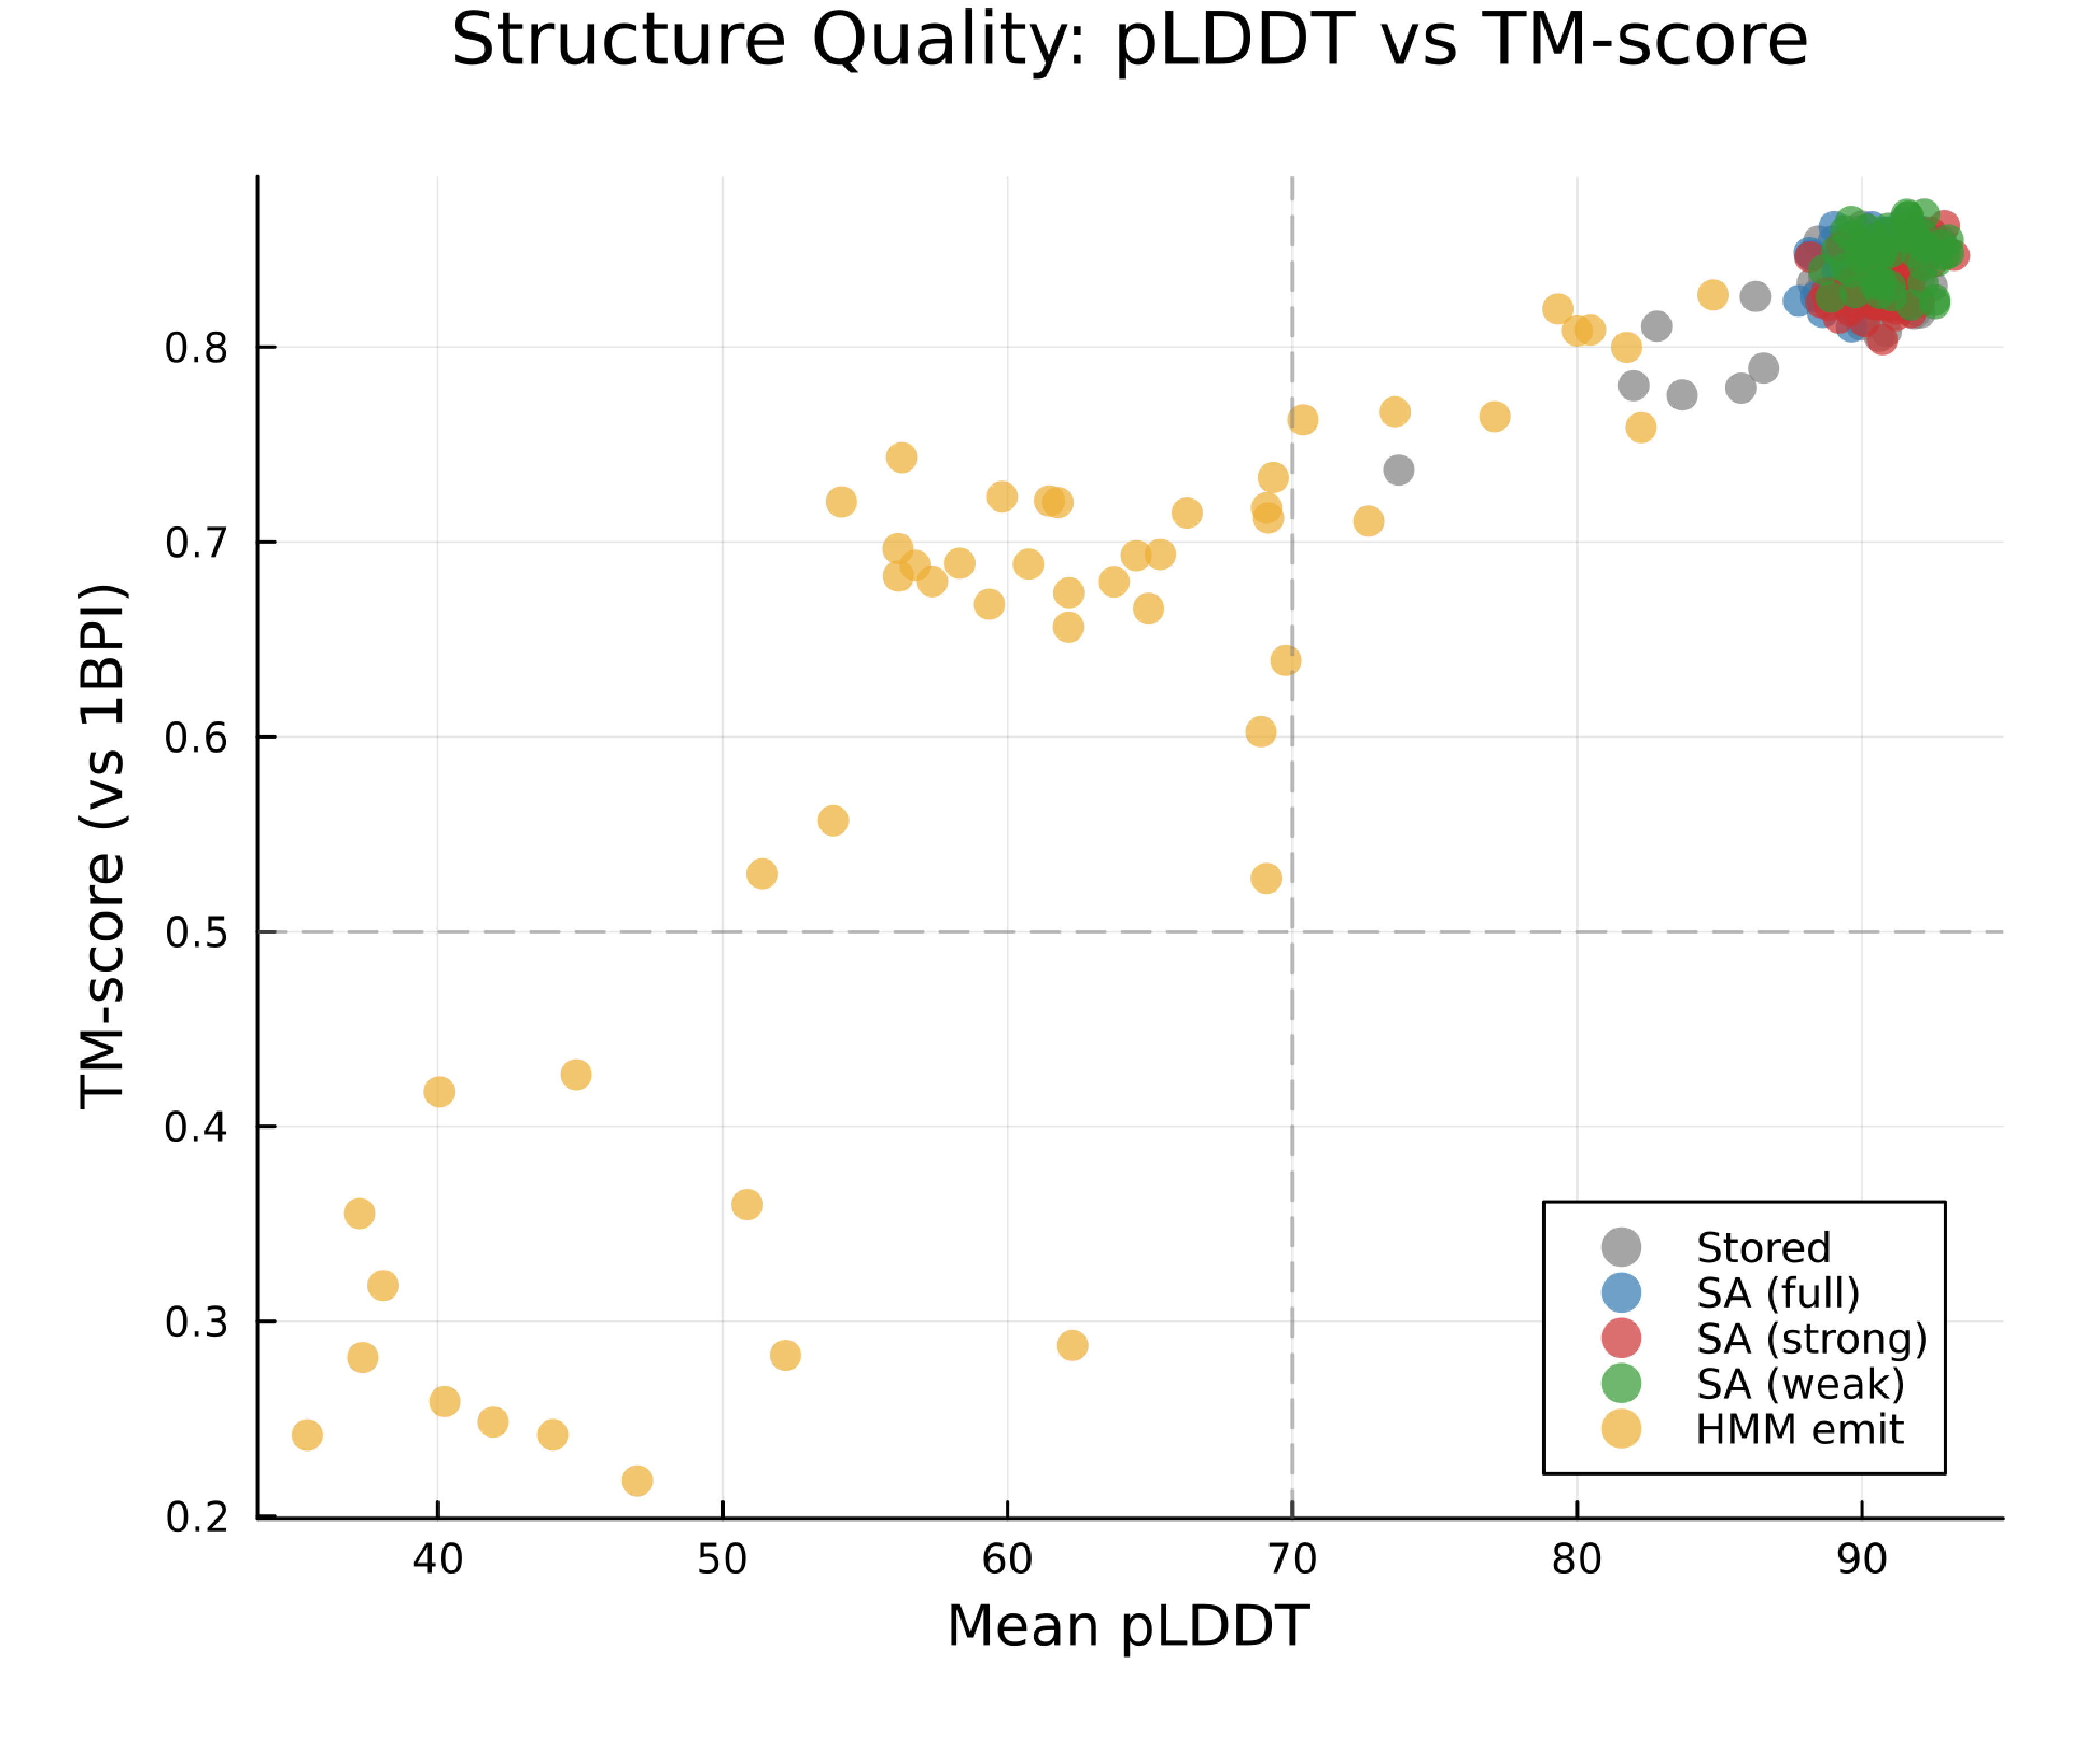
\includegraphics[width=0.72\textwidth]{sections/figs/plddt_vs_tmscore_scatter.pdf}
  \caption{\textbf{pLDDT and TM-score are positively correlated; SA sequences cluster in
  the high model-score region.}
  Each point represents one predicted structure (50 per source). Stored (gray) and SA-generated
  (blue, red, green) sequences cluster tightly above pLDDT $>85$ and TM-score $>0.8$ (upper
  right quadrant). HMM sequences (orange) scatter broadly, with many falling below the
  pLDDT $>70$ confidence threshold (vertical dashed line) and the TM-score $>0.5$ same-fold
  threshold (horizontal dashed line).}
  \label{fig:plddt-tmscore-scatter}
\end{figure}

\end{document}
